\documentclass[a4paper,12pt]{book} % nie: report!


\usepackage[T1,plmath]{polski} % lepiej to zamiast babel!
\usepackage[utf8]{inputenc} % w razie kłopotów spróbować: \usepackage[utf8x]{inputenc}
\usepackage{fancyhdr} % nagłówki i stopki
\usepackage{indentfirst} % WAŻNE, MA BYĆ!
\usepackage[pdftex]{graphicx} % to do wstawiania rysunków
\usepackage{amsfonts} % pakiety od AMS, ułatwiają składanie pewnych techniczno-matematcyznych rzeczy
\usepackage{amsmath} % to do dodatkowych symboli, przydatne
\usepackage{amssymb} % to też do dodatkowych symboli, też przydatne
\usepackage{amsthm}
\usepackage{enumitem}
\usepackage[pdftex,
            left=1.1in,right=1.1in,
            top=1.1in,bottom=1.1in]{geometry} % marginesy
\usepackage{float}
\usepackage[font=small,labelfont=bf]{caption}
\usepackage{svg}
\usepackage{booktabs}
\usepackage{array}
\usepackage{adjustbox}


\usepackage{csquotes}
\usepackage[backend=biber, style=numeric, citestyle=numeric, language=polish, sortlocale=pl_PL]{biblatex}
\addbibresource{../bibliografia.bib}

\usepackage[colorlinks=true]{hyperref} % odnośniki interaktywne w PDFie
\hypersetup{allcolors=blue}

\usepackage{listings}
\lstset{
    basicstyle=\footnotesize\tt,
    numbers=left,
    numberstyle=\tiny,
    frame=tb,
    tabsize=4,
    columns=fixed,
    showstringspaces=false,
    showtabs=false,
    keepspaces,
    commentstyle=\color{red},
    keywordstyle=\color{blue}
}
\newfloat{lstfloat}{htbp}{lolst}[chapter]
\floatname{lstfloat}{Listing}
\def\lstfloatautorefname{Listing}


\pagestyle{fancy}
\renewcommand{\chaptermark}[1]{\markboth{#1}{}}
\renewcommand{\sectionmark}[1]{\markright{\thesection\ #1}}
\fancyhf{}
\fancyhead[LE,RO]{\footnotesize\bfseries\thepage}
\fancyhead[LO]{\footnotesize\rightmark}
\fancyhead[RE]{\footnotesize\leftmark}
\renewcommand{\headrulewidth}{0.5pt}
\renewcommand{\footrulewidth}{0pt}
\addtolength{\headheight}{1.5pt}
\fancypagestyle{plain}{\fancyhead{}\cfoot{\footnotesize\bfseries\thepage}\renewcommand{\headrulewidth}{0pt}}

\linespread{1.25}



\begin{document}
\begin{titlepage}
\begin{tabular}{c@{\hspace{21mm}}|@{\hspace{5mm}}l}
\vspace{-20mm} & \\
\multicolumn{2}{l}{\hspace{-12.5mm} 
\includegraphics[width=8cm]{assets/LogoUMCS.jpg}} \\
\multicolumn{2}{@{\hspace{20mm}}l}{\vspace{-4mm}} \\
\multicolumn{2}{@{\hspace{28mm}}l}{\Large \sf UNIWERSYTET MARII
	CURIE-SKŁODOWSKIEJ} \\
\multicolumn{2}{@{\hspace{28mm}}l}{\vspace{-4mm}} \\
\multicolumn{2}{@{\hspace{28mm}}l}{\Large \sf W LUBLINIE} \\
\multicolumn{2}{@{\hspace{28mm}}l}{\vspace{-4mm}} \\
\multicolumn{2}{@{\hspace{28mm}}l}{\Large \sf Wydział Matematyki, Fizyki i
	Informatyki} \\
\multicolumn{2}{@{\hspace{28mm}}l}{\vspace{21mm}} \\
& {\sf Kierunek: \textbf{informatyka} } \\
& \\\\\\
& {\sf \large \bfseries Rafał Lenart} \\
& {\sf nr albumu: 307726} \\
& \\\\\\
& \Large \sf \bfseries Porównanie wydajności i ocena\\
& \Large \sf \bfseries łatwości użycia wybranych narzędzi\\
& \Large \sf \bfseries programowania równoległego \\\\[-10pt]
& {\large \sf Performance comparison and} \\
& {\large \sf ease of use assessment} \\
& {\large \sf of selected parallel programming tools} \\
& \\
& \\
& \\
& {\sf Praca licencjacka}  \\
& \vspace{-7mm} \\
&  {\sf napisana w Katedrze cyberbezpieczeństwa i lingwistyki komputerowej} \\
& \vspace{-7mm} \\
&  {\sf Instytutu Informatyki UMCS} \\
& \vspace{-7mm} \\
& {\sf pod kierunkiem \bfseries dr. hab. Jarosława Byliny} \\
\multicolumn{2}{@{\hspace{28mm}}l}{\vspace{15mm}} \\
\multicolumn{2}{@{\hspace{28mm}}l}{\textbf{\textsf{Lublin 2024}}}
\end{tabular}
\end{titlepage}





\sloppy



\thispagestyle{empty}


\newpage{}

\thispagestyle{empty}

\newpage{}



\tableofcontents{}

\chapter*{Wstęp}
\addcontentsline{toc}{chapter}{Wstęp}
Na przestrzeni lat powstało wiele narzędzi mających za zadanie umożliwić programowanie równoległe. Wraz z rosnącą liczbą możliwych do wyboru opcji często pojawiają się pytania na temat relatywnej wydajności takich rozwiązań. Zważając na fakt, że równoleglizacja operacji wykonywanych przez program często nie jest rzeczą łatwą oraz zwiększa ilość czasu potrzebną do implementacji rozwiązania różnych problemów, zaczęły powstawać narzędzia które próbują skrócić ten proces oraz zwiększyć produktywność, zachowując przy tym odpowiedni poziom wydajności. 

Celem tej pracy jest porównanie wydajności oraz łatwości w użyciu trzech takich narzędzi. Opracowaliśmy w niej programy z użyciem narzędzi SYCL, MPI oraz biblioteki Distributed Ranges. Wykonaliśmy testy polegające na porównaniu ich wydajności oraz łatwości w użyciu implementując rozwiązania trzech problemów: całkowania metodą Monte Carlo, rozwiązywania układu równań liniowych z pomocą metody gradientu sprzężonego oraz obliczanie szybkiej transformacji Fouriera. 

Najpierw opisaliśmy kilka ważnych pojęć związanych z programowaniem równoległym. Drugi rozdział przedstawia pokrótce narzędzia oraz algorytmy wybrane jako obiekt testów oraz opisuje środowsko na którym zostały one przeprowadzone. W kolejnym rozdziale znajduje się opis problemów napotkanych przy implementacji oraz krótki komentarz na temat ostatecznych wyników testu. Rozdział czwarty zawiera opinię na temat łatwości w użyciu wybranych do porównania narzędzi. Piąty rozdział w większych szczegółach przedstawia wyniki wykonanych testów oraz wnioski które można z nich wyciągnąć. Ostatni rozdział jest podsumowaniem wyników projektu.

\chapter{Programowanie równoległe}
W świecie dzisiejszej informatyki oraz technologii obliczeniowych kluczowym wyzwaniem jest wykonywanie obliczeń na bardzo dużych zbiorach danych. Sekwencyjne podejście do takich problemów stało się niewystarczające. W obliczu ciągle rosnących wymagań obliczeniowych współczesnego świata zaszła potrzeba przyspieszenia niektórych operacji. W ten sposób powstała idea programowania równoległego, które pozwala na wykorzystanie wielu jednostek obliczeniowych do jednoczesnego wykonywania obliczeń.

Programowanie równoległe polega na podziale zadania na mniejsze, niezależne od siebie części, które mogą być przetwarzane jednocześnie. Wykorzystanie kart graficznych oraz procesorów wielordzeniowych prowadzi do znacznego skrócenia czasu wykonywania zadań.

Celem tego rozdziału jest omówienie podstawowych koncepcji związanych z programowaniem równoległym oraz wprowadzenie terminologii.

\section{Podstawowe pojęcia}
W tym podrozdziale wymienionych zostanie kilka podstawowych pojęć często używanych w kontekscie programowania równoległego.
\begin{itemize}
\item Proces - działający program, dla którego system operacyjny zarezerwował zasoby. W jednym procesie może istnieć wiele wątków.
\item Wątek - część programu wykonywana współbieżnie w obrębie jednego procesu. Utworzenie wątku jest o wiele szybsze niż utworzenie procesu.
\item Bariera - w kontekście programowania równoległego jest to mechanizm synchronizacyjny powodujący, że wątki czekają na siebie, zanim przejdą do kolejnych obliczeń.
\item Mutex (ang. \emph{mutual exclusion}, wzajemne wykluczenie) - Narzędzie synchronizacyjne kontroli dostępu do współdzielonego przez wiele wątków zasobu.
\item Wyścig danych (ang. \emph{race condition}) - Sytuacja w której dochodzi do błędu wywołanego niekontrolowanym porządkiem wykonywania obliczeń.
\item Zakleszczenie (ang. \emph{deadlock}) - Stan w którym dwa lub więcej wątków oczekuje na zasoby w sposób uniemożliwiający kontynuowanie ich pracy.
\item Zawstydzająca równoległość - Mówimy, że algorytm jest zawstydzająco równoległy, jeśli pomiędzy podzadaniami wydzielonymi dla różnych wątków nie zachodzi potrzeba kontaktu. Takie problemy są najłatwiejsze w implementacji.
\item Wielowątkowość współbieżna (ang. \emph{Simultaneous Multi-Threading}, SMT) - to technika poprawy wydajności procesora poprzez umożliwienie wykonywania niezależnych od siebie wątków na jednym rdzeniu.
\end{itemize}

\section{Taksonomia Flynna}
Taksonomia Flynna to klasyfikacja systemów komputerowych zaproponowana przez Michaela J. Flynna w 1996 roku \cite{Flynn1966}. System klasyfikacji uwzględnia jako czynniki liczbę strumieni rozkazów oraz liczbę strumieni danych.
W pierwotnej wersji Flynn opisał cztery klasy systemów komputerowych. Zaliczają się do nich:
\begin{itemize}[topsep=1pt, itemsep=0.5pt]
	\item pojedynczy strumień rozkazów, pojedynczy strumień danych (ang. \emph{single instruction, single data, SISD});
	\item pojedynczy strumień rozkazów, wiele strumieni danych (ang. \emph{single instruction, multiple data, SIMD});
	\item wielokrotny strumień rozkazów, pojedynczy strumień danych (ang. \emph{multiple instruction, single data, MISD});
	\item wielokrotny strumień rozkazów, wiele strumieni danych (ang. \emph{multiple instruction, multiple data, MIMD}).
\end{itemize}

\subsection{SISD}
W grupie SISD znajdują się komputery sekwencyjne, nie wykorzystujące zrównoleglenia w strumieniu danych, ani w strumieniu rozkazów. Pojedyncza jednostka sterująca przetwarza jeden strumień danych jednym rozkazem. W tej grupie znajdują się komputery w architekturze von Neumanna \cite{Neumann}. Przykładem systemów SISD mogą być komputery wykorzystujące jeden procesor (z jednym rdzeniem) do wykonywania wszystkich operacji. Rysunek \ref{fig:sisd} obrazuje architekturę SISD w postaci diagramu.
\begin{figure}
	\centering
	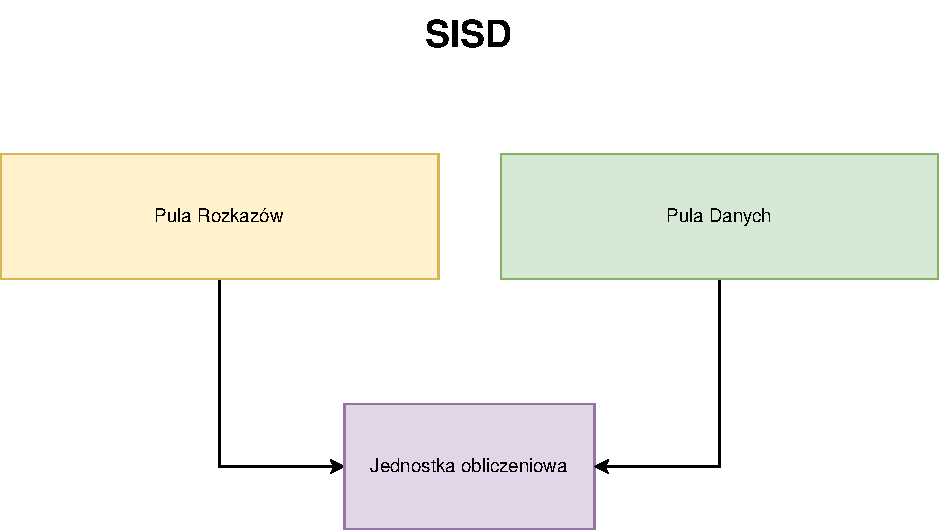
\includegraphics[scale=1]{assets/SISD.pdf}
	\caption{Diagram SISD.}
	\label{fig:sisd}
\end{figure}

\subsection{SIMD}
W komputerach z kategorii SIMD instrukcje mogą być wykonywane sekwencyjne lub równolegle przez kilka jednostek funkcyjnych. W artykule Flynna z roku 1972 \cite{Flynn1972} autor dokonał dodatkowego podziału klasy na trzy podkategorie:
\begin{itemize}
	\item Procesor wektorowy (ang. \emph{Array processor}) - obliczenia są wykonywane na całych wektorach danych, każda jednostka obliczeniowa posiada własny rejestr pamięci.
	\item Procesor potokowy (ang. \emph{Pipelined processor}) - jednostka obliczeniowa wykonuje instrukcje na fragmencie danych z centralnej jednostki pamięci i przetworzone dane zapisuje do tej samej jednostki.
	\item Procesor asocjacyjny (ang. \emph{Associative processor}) - tego typu systemy otrzymują ten sam rozkaz, jednak każda jednostka obliczeniowa podejmuje niezależną decyzję odnośnie tego czy wykonać zadaną instrukcję, czy ją pominąć. Decyzja ta jest podejmowana na podstawie danych otrzymanych przez daną jednostkę.
\end{itemize}
Superkomputery wektorowe są głównymi reprezentantami kategorii SIMD. Bardzo popularnym przykładem jest Cray-1 \cite{Cray-1}, superkomputer z lat siedemdziesiątych który obecnie znajduje się w Muzeum Nauki w Londynie. W wielu współczesnych architekturach procesorów są dostępne instrukcje które wykonują operacje wektorowe. Rysunek \ref{fig:simd} obrazuje architekturę SIMD w postaci diagramu.
\begin{figure}
	\centering
	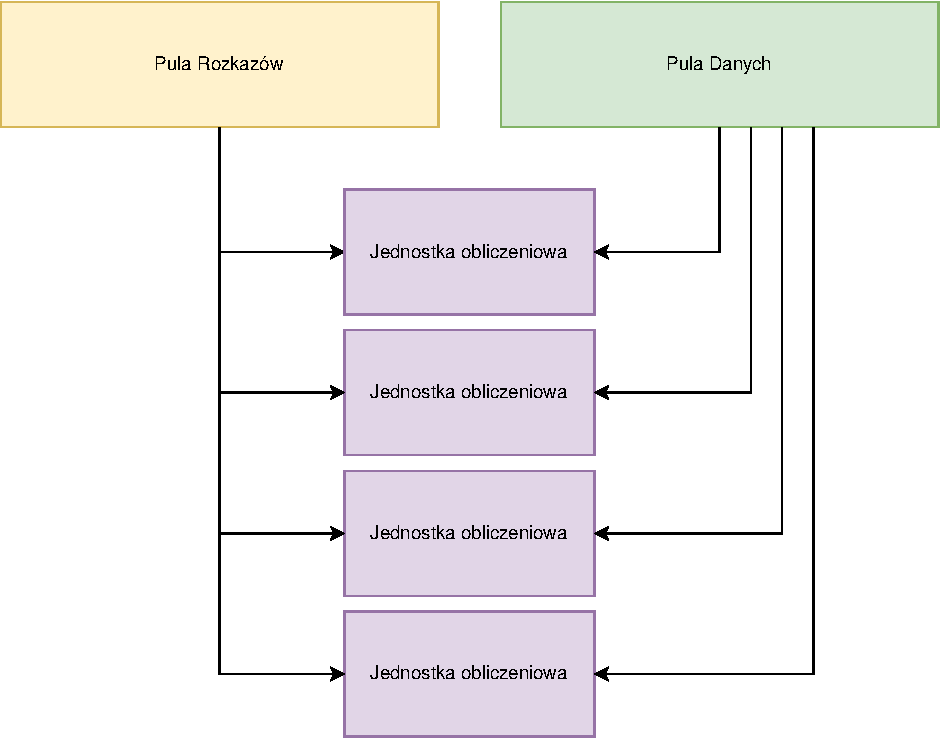
\includegraphics[scale=1]{assets/SIMD.pdf}
	\caption{Diagram SIMD.}
	\label{fig:simd}
\end{figure}

\subsection {MISD}
MISD jest architekturą stosowaną niezwykle rzadko, gdyż jedynym jej zastosowaniem jest minimalizacja błędów poprzez wykonywanie tej samej instrukcji wielokrotnie. Dobrze znanym przypadkiem użycia jest komputer Wahadłowca Kosmicznego skonstruowanego przez NASA \cite{SpaceShuttle}. Rysunek \ref{fig:misd} obrazuje architekturę MISD w postaci diagramu.
\begin{figure}
	\centering
	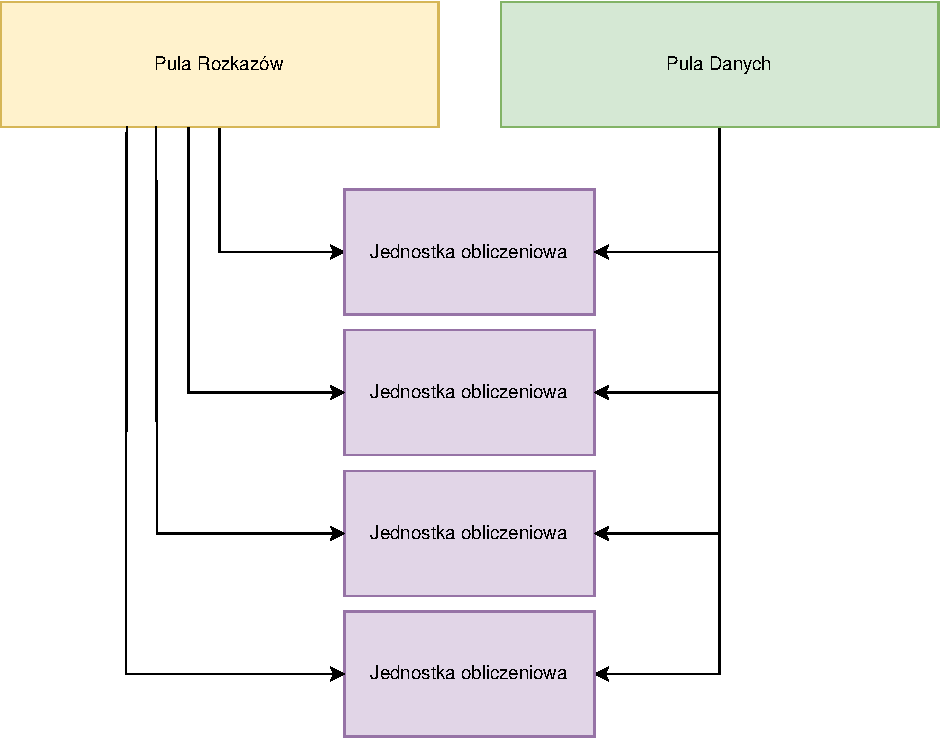
\includegraphics[scale=1]{assets/MISD.pdf}
	\caption{Diagram MISD.}
	\label{fig:misd}
\end{figure}

\subsection {MIMD}
MIMD to architektura, pozwalająca na wykonywanie wielu instrukcji na wielu strumieniach danych. Jest to obecnie najbardziej popularna klasa komputerów. Nowoczesne komputery osobiste najczęściej posiadają wielordzeniowe procesory, które mają możliwość równoległego wykonywania różnych instrukcji na róznych zestawach danych. Rysunek \ref{fig:mimd} obrazuje architekturę MIMD w postaci diagramu.
\begin{figure}
	\centering
	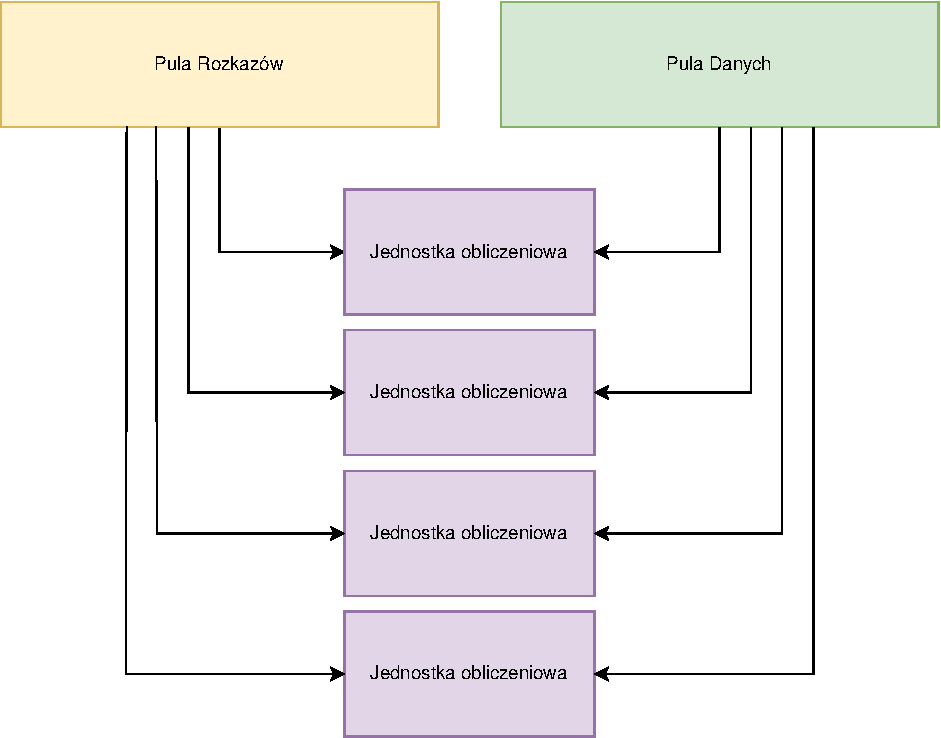
\includegraphics[scale=1]{assets/MIMD.pdf}
	\caption{Diagram MIMD.}
	\label{fig:mimd}
\end{figure}

\section{Pamięć komputera}
W systemach równoległych istnieją dwa modele organizacji pamięci:
\begin{itemize}
	\item Pamięć wspólna - wszystkie procesory w tym modelu mają dostęp do wspólnej przestrzeni adresowej. To rozwiązanie często może być wolniejsze poprzez jednoczesne próby dostępu do pamięci przez poszczególne jednostki. Dużą zaletą tego typu architektury jest łatwa komunikacja pomiędzy procesorami.
	\item Pamięć rozproszona - każdy z procesorów w tym modelu posiada pamięć lokalną, a komunikacja między nimi zachodzi przez sieć. Zaletą tego rozwiązania jest duża skalowalność oraz brak problemu jednoczesnego dostępu do pamięci. Niestety, niedogodnością jest konieczność stosowania bardziej skomplikowanych mechanizmów komunikacji oraz często wyspecjalizowanych algorytmów stworzonych dokładnie do tego celu.
\end{itemize}
Duże znaczenie we współczesnych systemach komputerowych odgrywają również różne rodzaje pamięci \cite{hierarchia-pamieci}.
\begin{itemize}
	\item Pamięć masowa/drugorzędna - pamięć długoterminowa zachowująca stan nawet po odłączeniu od źródła zasilania. Jest to najbardziej pojemny, ale i najwolniejszy rodzaj pamięci. W większości przypadków fizycznie znajduje się najdalej od procesora.
	\item Pamięć operacyjna, pamięć o dostępie swobodnym (ang. \emph{Random Access Memory}, RAM) - rodzaj pamięci znajdujący się blisko procesora, aby umożliwić duże prędkości przesyłu danych. Ma mniejszą pojemność niż pamięć masowa.
	\item Pamięć podręczna (ang. \emph{Cache memory}) - najszybsza pamięć, która przechowuje dane do których jest potrzebny bardzo szybki dostęp. Fizycznie często jest zintegrowana bezpośrednio z procesorem. Ma ona małą pojemność i to z niej procesor pobiera dane do swoich rejestrów.
	\item Rejestry procesora - jednostki pamięci na których bezpośrednio są wykonywane operacje.
\end{itemize}
W dzisiejszych czasach, rodzajem pamięci decydującym o prędkości wykonywanych operacji jest pamięć podręczna. Algorytmy oraz struktury danych, z których korzysta program, powinny być dobierane tak, aby zminimalizować konieczność częstego przenoszenia danych z RAM do pamięci podręcznej.
Hierarchia pamięci zwizualizowano na rysunku \ref{fig:hierarchia_pamieci} \cite{cache-memory}.
\begin{figure}[h]
	\centering
	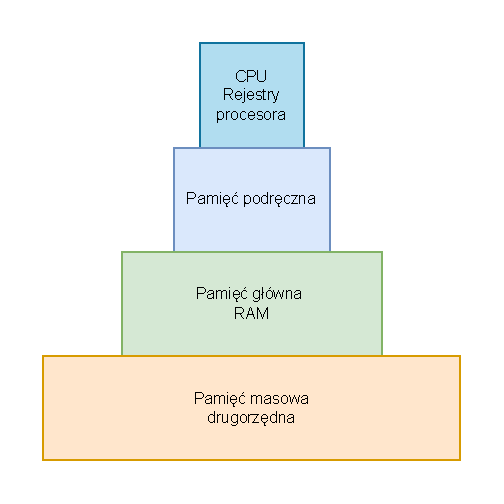
\includegraphics[scale=1]{assets/hierarchia_pamieci.pdf}
	\caption{Hierarchia pamięci.}
	\label{fig:hierarchia_pamieci}
\end{figure}

\chapter{Przegląd wykonanych testów}
Ten rozdział zawiera opis narzędzi oraz problemów które poddano testom wydajności oraz łatwości w użyciu. Dodatkowo w ostatnim podrozdziale zawarty jest opis środowiska, na którym przeprowadziliśmy wszystkie badania.
\section{Wybrane narzędzia}
Narzędzia, które wybraliśmy do porównania to SYCL, MPI (ang. \emph{Message Passing Interface}) oraz biblioteka Distributed Ranges wykorzystująca obydwie te technologie \cite{SYCL, MPI, dist-ranges}. Distributed Ranges przygotowana przez jeden z zespołów firmy Intel jako cel obrała zwiększenie produktywności pracy programistów przy pisaniu kodu. Motywacją dokonania tego wyboru jest chęć sprawdzenia obecnego stanu rozwoju. MPI oraz SYCL wybraliśmy ze względu na to, że Distributed Ranges w dużej mierze bazuje na tych dwóch technologiach.
\subsection{SYCL}
Na stronie internetowej grupy Khronos, twórców narzędzia, widnieje zdanie: ,,SYCL to bezpłatna, wieloplatformowa warstwa abstrakcji [...]''\cite{SYCL-overview}. Jest on modelem zgodnym ze standardem C++ 17. Jego zadaniem i głównym celem jest umożliwienie współpracy wielu urządzeniom w jednej aplikacji. Twórcom udaje się to poprzez udostępnienie API (ang. \emph{Application Programming Interface}, interfejsów programistycznych aplikacji) oraz abstrakcji dających dostęp do urządzeń takich jak procesory, karty graficzne czy FPGA (ang. \emph{Field Programmable Gate Array}, bezpośrednio programowalne macierze bramek). SYCL jest więc modelem wysokopoziomowym, używającym nowoczesnych standardów, który upraszcza działanie z wieloma urządzeniami na raz. Wstępna specyfikacja SYCL została udostępniona 19 marca 2014 roku \cite{SYCL1.2-provisional}. Finalną specyfikację SYCL 1.2 wydano ponad rok później, 11 maja 2015 roku \cite{SYCL1.2}. Obecnie najnowszym wydaniem specyfikacji jest SYCL 2020 z 9 lutego 2021 roku. Istnieje kilka rozwijanych równolegle implementacji modelu SYCL. W projekcie użyliśmy rozwiązania firmy Intel zawartego w zestawie narzędzi oneAPI.
\subsection{MPI}
Interfejs przekazywania wiadomości (ang. \emph{Message Passing Interface}, MPI) jest standardem przenoszenia informacji pomiędzy procesami programów równoległych. Ten protokół komunikacyjny utworzony i ustandaryzowany w czerwcu 1994 roku jest rezultatem prac wielu osób oraz firm. MPI jest szeroko wykorzystywany przy tworzeniu programów działających w systemach z pamięcią rozproszoną. Wiele języków programowania posiada własne implementacje MPI, jednak najczęściej używanymi są kompilatory języków C, C++ oraz Fortran. Standard od czasu swojego powstania był wciąż rozwijany i powstało kilka wersji, które bazowały i wzbogacały swoich poprzedników o nowe funkcje. Najnowszą zatwierdzoną przez forum wersją jest MPI-4.1 z listopada 2023 roku \cite{mpi41}.
\subsection{Distributed Ranges}
Zakresy rozproszone (ang. \emph{Distributed Ranges}) to biblioteka języka C++ utworzona przez firmę Intel zwiększająca produktywność pracy w systemach z pamięcią rozproszoną. Narzędzie to wykorzystuje bibliotekę ranges ze standardu C++ 20 i oferuje kolekcję struktur danych, widoków oraz algorytmów. Distributed ranges jest kompatybilna i zdolna do współpracy z MPI, SYCL, OpenMP oraz SHMEM. Kod źródłowy biblioteki jest otwarty i dostępny za darmo \cite{dist-ranges}. Repozytorium powstało i jest rozwijane od 2022 roku. Jako, że zarówno biblioteka ranges (C++20), jak i Distributed Ranges, są technologiami wprowadzonymi niedawno, postaramy się przybliżyć najważnejsze informacje z nimi związane.
\subsubsection{Ranges}
Nagłówek \emph{<ranges>} zawiera kilka konceptów (ang. \emph{concept}), które są, w najprostszej swojej postaci, abstrakcją dowolnego, iterowalnego zbioru elementów posiadającego początek i koniec \cite{ranges}. Kolekcja ta, aby spełnić bazową definicję \emph{range}, musi posiadać metody \emph{begin()} oraz \emph{end()}. W tabeli \ref{ranges_concepts} znajduje się krótki opis kilku konceptów z \emph{std::ranges} oraz informacja o tym które z najczęściej używanych struktur danych z STL (ang. \emph{Standard Template Library}, Standardowa biblioteka szablonów) spełniają dany koncept.
\begin{table}[H]
\begin{adjustbox}{max width=\textheight, angle=90, center}
\begin{tabular}{|l|m{7cm}|ccccc|}
\hline
	& Opis & \texttt{std::forward\_list} & \texttt{std::list} & \texttt{std::deque} & \texttt{std::array} & \texttt{std::vector} \\
\hline
\texttt{std::ranges::output\_range} & Może iterować do przodu & X & X & X & X & X \\
\hline
\texttt{std::ranges::input\_range} & Można iterować po nim od początku do końca przynajmniej raz & X & X & X & X & X \\
\hline
\texttt{std::ranges::forward\_range} & Można iterować po nim od początku do końca wielokrotnie & X & X & X & X & X \\
\hline
\texttt{std::ranges::bidirectional\_range} & Iterator może poruszać się do tyłu & & X & X & X & X \\
\hline
\texttt{std::ranges::random\_access\_range} & Dostęp do każdego elementu jest w czasie stałym & & & X & X & X \\
\hline
\texttt{std::ranges::contiguous\_range} & Elementy są przechowywane w pamięci jeden po drugim & & & & X & X \\
\hline
\end{tabular}
\end{adjustbox}
\caption{Wybrane koncepty z std::ranges}
\label{ranges_concepts}
\end{table}
W bibliotece zdefiniowane są klasy widoków (ang. \emph{view}). Widok to zakres odwołujący się do elementów, których nie posiada. Widok jest sposobem modyfikacji zakresu, do którego się odwołuje. Łączenie i tworzenie widoków jest bardzo wydajne, gdyż uzyskiwanie dostępu do elementów widoku odbywa się "leniwie", czyli tak, aby operacje wykonano dopiero przy próbie dostępu do wartości. Przykładem wykorzystania zakresów może być listing \ref{lst:ranges_przyklad}. Jak widać, widoki można łączyć ze sobą aby w prosty i wydajny sposób, aby wykonywać większe, bardziej skomplikowane operacje. Odbywa się to często poprzez użycie operatora potoku "$|$", analogicznego do tego występującego w powłoce Bash.

\begin{lstfloat}[H]
\lstset{language=C++}
\begin{lstlisting}[frame=single]
#include <ranges>
#include <vector>
#include <iostream>

int main() {
	std::vector<int> input =  {0, 1, 2, 3, 4, 5, 6, 7, 8, 9};
    auto is_even = [](const int val) {return val % 2 == 0;};
    auto times_two = [](const int val) {return val * 2;};

    auto result = input
             | std::views::filter(is_even)
             | std::views::transform(times_two);
    
    std::cout << "Wynik: ";
    for (int val : result) {
    		std::cout << val << ' ';
  	}
}

Wynik: 0 4 8 12 16
\end{lstlisting}
\caption{Przykład użycia biblioteki \emph{ranges}}\label{lst:ranges_przyklad}
\end{lstfloat}

\subsubsection{Distributed Ranges}
Podobnie jak opisana wyżej biblioteka z C++20, Distributed Ranges wprowadza kilka konceptów, na których oparte są struktury. Najważniejszym z tych konceptów jest \texttt{distributed\_range} opisany tak jak na listingu \ref{lst:distributed_range}, w pliku \emph{concepts.hpp}.

\begin{lstfloat}[H]
\lstset{language=C++}
\begin{lstlisting}[frame=single]
template <typename R>
concept distributed_range =
  rng::forward_range<R> && requires(R &r) { dr::ranges::segments(r); };
\end{lstlisting}
\caption{Koncept \texttt{distributed\_range}}
\label{lst:distributed_range}
\end{lstfloat}

Ponadto, biblioteka jest podzielona na dwie przestrzenie nazw czyli \texttt{dr::mhp} oraz \texttt{dr::shp}. Na potrzeby naszego projektu bardziej interesującą częścią biblioteki jest zdecydowanie mhp. Są w niej zdefiniowane dwie struktury danych: \texttt{dr::mhp::distributed\_vector} oraz \texttt{dr:mhp::distributed\_dense\_matrix}. Operacje udostępnione dla tych struktur mogą być wykorzystywane do programowania systemów komputerowych z pamięcią rozproszoną poprzez użycie połączenia MPI oraz SYCL. Druga część biblioteki pozwala, tak jak mhp oraz SYCL, na wykorzystanie kilku CPU/GPU, jednak w jednym procesie i tylko na jednym węźle. \texttt{dr::shp} jest bardziej rozwinięta i posiada więcej funkcji oraz narzędzi które jeszcze nie są zaimplementowane w mhp. Dla obu części istnieje obecnie zbiór widoków pozwalających na przeprowadzanie operacji w sposób identyczny jak w \texttt{<ranges>}.




\section{Wybrane algorytmy}
Aby porównać wydajność i łatwość w użyciu narzędzi opisanych w poprzednim podrozdziale, koniecznym jest dobór algorytmów których implementacje będą poddawane testom. Problemy które wybraliśmy na potrzeby projektu to
\begin{itemize}
\item całkowanie metodą Monte Carlo,
\item metoda gradientu sprzężonego,
\item szybka transformacja Fouriera.
\end{itemize}
W dalszej części opisaliśmy te zagadnienia w kolejności od najprostszego w implementacji do najtrudniejszego.
\subsection{Całkowanie metodą Monte Carlo}
Metodami Monte Carlo nazywamy techniki i algorytmy uzyskiwania wyników operacji numerycznych poprzez wielokrotne losowe próbkowanie. Głównym twórcą metody był polski fizyk Stanisław Ulam, który zainspirowany hazardowymi nawykami swojego wujka nadał jej nazwę pochodzącą od kasyna Monte Carlo w Monako \cite{mc_beggining}.
Obliczanie całki tą metodą to bardzo prosta operacja. Wystarczy wylosować dostateczną liczbę punktów z podanego zakresu aby zapewnić wysoką dokładność wyniku i dla każdego z nich sprawdzić czy znajduje się on pod wykresem sprawdzanej funkcji. Dokładność wyników otrzymanych przy użyciu tej metody zależy w dużej mierze od parametrów wybranego generatora liczb pseudolosowych.
W projekcie obliczamy całkę funkcji stu-wymiarowej, co sprowadza się do obliczenia miary Jordana \cite{miara-jordana} stu-wymiarowej przestrzeni pod funkcją. Jako zakres całkowania przyjęliśmy hipersześcian, współdzielący środek z układem współrzędnych. Zdecydowaliśmy się na taki zabieg po to, aby zwiększyć ilość obliczeń, a tym samym czas wykonywania programu. 
\subsection{Metoda gradientu sprzężonego}
Metoda gradientu sprzężonego (ang. \emph{conjugate gradient method}, CG) jest metodą numeryczną zaproponowaną w 1952 roku \cite{conjugate-gradient}, pozwalającą na rozwiązywanie układów równań liniowych w postaci $Ax = b$, których macierz $A$ spełnia następujące warunki:
\begin{itemize}
\item jest symetryczna $A^T=A$ co oznacza, że dla każdego $i, j$ prawdziwe jest równanie $a_{ij} = a_{ji}.$
\item jest dodatnio określona.
\end{itemize}

Symetryczność macierzy jest cechą dobrze znaną, jednak aby przybliżyć cechę dodatniej określoności należy wprowadzić kilka pojęć.

\newtheorem{df}{Definicja} 
\theoremstyle{definition}
\begin{df} 
Formą kwadratową\cite{quadratic-form}, nazywamy wielomian, którego każda zmienna jest drugiego stopnia. Możemy ją uprościć do postaci:
$$f(x) = x^TAx,$$
gdzie $A$ jest macierzą symetryczną, zwaną macierzą formy kwadratowej $f$. Jeżeli przyjmiemy $A = [a_{ij}]$ to równoważną formą jest
$$f(x_1,x_2,\ldots,x_n) = \sum_{i=1}^n\sum_{j=1}^na_{ij}x_ix_j.$$
\end{df}

\begin{df} 
Mówimy, że forma kwadratowa nad rzeczywistą przestrzenią liniową $V$ jest określona, jeżeli przyjmuje wartości tego samego znaku dla wszystkich punktów $x$ tej przestrzeni liniowej. Dodatkowo spośród form określonych można wyróżnić:
\begin{enumerate}
\item $\forall x \in \mathbb{R}^n/\{0\}: f(x) > 0$ - formę dodatnio określoną, oraz
\item $\forall x \in \mathbb{R}^n/\{0\}: f(x) < 0$ - formę ujemnie określoną.  
\end{enumerate}
Jeżeli natomiast forma jest równa zero dla wszystkich wartości $x$ to nazywamy ją zdegenerowaną.
\end{df}

\begin{df}
Symetryczną macierz $A$ nazywamy dodatnio określoną kiedy jest macierzą dodatnio określonej formy kwadratowej $f(x) = x^TAx$.
\end{df}

Oznaczmy rozwiązanie układu $Ax = b$ jako $x_*.$

\begin{df}
Dwa niezerowe wektory $u$ i $v$ są sprzężone względem macierzy A, jeżeli spełniają równanie $u^TAv = 0.$
\end{df}

Przyjmując jako warunek symetryczność oraz dodatnią określoność macierzy możemy zapisać iloczyn skalarny:
$$u^TAv = \langle u,Av\rangle = \langle Au, v \rangle = \langle A^Tu, v \rangle = \langle u, v \rangle_A.$$
Znając warunek ortogonalności wektorów $\langle u, v\rangle = 0$ można zauważyć, że dwa wektory są wzajemnie sprzężone jeżeli są ortogonalne względem iloczynu skalarnego $\langle u, v \rangle_A.$


\begin{df}
Kombinacją liniową układu wektorów $x_1, \ldots,x_n$ o współczynnikach $\alpha_1,\ldots,\alpha_n$ nazywamy wektor
$$ x = \sum_{i=1}^n\alpha_ix_i = \alpha_1x_1 + \alpha_2x_2 + \ldots + \alpha_nx_n.$$
\end{df}

\begin{df}
Mówimy, że ciąg wektorów $v_1, v_2, \ldots, v_k$ z przestrzeni $V$ jest liniowo niezależny, gdy równanie $$a_1v_1 + a_2v_2 + \ldots + a_kv_k = \mathbf{0},$$ gdzie $\mathbf{0}$ oznacza wektor zerowy, jest spełnione tylko w przypadku gdy $a_i = 0$ dla $i = 1, 2, \ldots, k.$
\end{df}

\begin{df} 
Zbiór wektorów $B$ należacych do jakiejś przestrzeni $V$ spełniający dwa warunki:
\begin{enumerate}
\item Generuje przestrzeń $V$, to znaczy każdy wektor z przestrzeni $V$ może być zapisany jako kombinacja liniowa wektorów ze zbioru $B;$
\item jest liniowo niezależny;
\end{enumerate}
nazywamy bazą przestrzeni wektorowej $V$.
\end{df}


Załóżmy, że $P = \{p_1, p_2, \ldots, p_n\}$ jest ciągiem $n$ parami sprzężonych względem $A$ kierunków, czyli 
$$\forall i \neq j: p_i^TAp_j = 0 .$$

\newtheorem{thm}{Twierdzenie} 
\theoremstyle{definition}
\begin{thm}
$P$ stanowi bazę $\mathbb{R}^n.$
\end{thm}
\begin{proof}
Załóżmy, że istnieje kombinacja liniowa układu $P$ z conajmniej jednym niezerowym współczynnikiem $\alpha_i$ dająca wektor zerowy:
$$\alpha_1p_1 + \alpha_2p_2 + \ldots + \alpha_np_n = 0.$$
Aby udowodnić, że $\alpha_i = 0$ dla wszystkich $i=1,\ldots,n$ przemnóżmy powyższą kombinację obustronnie przez $p_i^TA.$
$$p_i^TA(\alpha_1p_1 + \alpha_2p_2 + \ldots + \alpha_np_n) = p_i^TA0 = 0$$
$$\sum_{j=1}^n\alpha_jp_i^TAp_j = 0$$
Wykorzystując wzajemną sprzężoność wektorów $p_i^TAp_j = 0$ dla $i \neq j$ otrzymujemy:
$$\alpha_ip_i^TAp_i = 0.$$ 
Ponieważ A jest macierzą dodatnio określoną, to $p_i^TAp_i \neq 0,$ dzięki temu można zapisać: $$\alpha_i = 0.$$ 
\end{proof}


Zatem wektor wynikowy $x_*$ możemy przedstawić w postaci $x_* = \sum_{i=1}^n\alpha_ip_i.$ podstawiając to do układu równań $Ax = b$ otrzymujemy:
$$ Ax_* = \sum^n_{i=1}\alpha_iAp_i = b. $$ Wymnożenie tego równania przez wektor $p_k^T$ daje nam:
$$p_k^Tb = \sum_{i=1}^n\alpha_ip_k^TAp_i = \sum_{i=1}^n\alpha_i\langle p_k, p_i\rangle_A.$$
Wiedząc, że $\langle p_k, p_i \rangle_A = 0$ dla każdego $k \neq i$ możemy dalej uprościć równanie do postaci:
$$p_k^Tb = \alpha_k\langle p_k, p_k\rangle_A,$$ 
a więc
$$ \alpha_k = \frac{\langle p_k, b \rangle }{\langle p_k, p_k \rangle_A}. $$
Otrzymujemy w ten sposób metodę rozwiązywania $Ax = b.$ Należy znaleźć ciąg $n$ sprzężonych kierunków po czym obliczyć wpółczynniki $\alpha_k.$

Odpowiednie dobranie wektorów $p_k,$ może sprawić, że nie będziemy potrzebowali ich wszystkich do uzyskania wystarczająco dobrego przybliżenia wyniku $x_*.$

\begin{df}
Gradientem funkcji $f$ nazywamy:
\[
f'(x) = 
\begin{bmatrix}
\frac{\partial }{\partial x_1}f(x) \\
\frac{\partial }{\partial x_2}f(x) \\
\vdots \\
\frac{\partial }{\partial x_n}f(x) \\
\end{bmatrix}
.
\]
\end{df}
Gradient, to wektor, który dla danego punktu $x$, wskazuje kierunek największego przyrostu $f(x)$.

Rozpatrzmy formę kwadratową o postaci $$f(x) = \frac{1}{2}x^TAx - b^Tx + c.$$ Można dokonać przekształceń \cite{gradient-quadratic, gradient-quadratic2}, które
doprowadzą nas do wzoru $f'(x) = \frac{1}{2}(A^T + A)x - b$ gradientu tej funkcji, co dla macierzy symetrycznej daje
$$f'(x) = Ax - b.$$

Przyjmijmy $x_0 = 0$ jako punkt startowy. Da się zauważyć, że rozwiązanie $x_*$ minimalizuje formę kwadratową. Załóżmy, że $x$ jest punktem który rozwiązuje $Ax = b$ oraz minimalizuje formę kwadratową w postaci $f(x) = \frac{1}{2}x^TAx - b^Tx + c$ oraz przyjmijmy $\alpha$ jako dowolny wyraz. Wtedy otrzymujemy
\begin{align*}
f(x + \alpha) &= \frac{1}{2}(x + \alpha)^TA(x+\alpha)-b^T(x+\alpha)+c \\
	&= \frac{1}{2}x^TAx+\alpha^TAx+\frac{1}{2}\alpha^TA\alpha-b^Tx - b^T\alpha+c \\
	&= \frac{1}{2}x^TAx-b^Tx+c+\alpha^Tb+\frac{1}{2}\alpha^TA\alpha -b^T\alpha \\
	&= f(x) + \frac{1}{2}\alpha^TA\alpha.
\end{align*}
Jeżeli A jest dodatnio określona to $\alpha^TA\alpha = 0,$ a więc $x$ minimalizuje $f.$
Ten fakt sugeruje aby jako pierwszy wektor bazowy $p_1$ wybrać gradient w $x_0,$ który po podstawieniu do wzoru wynosi $-b.$ Pozostałe wektory w bazie będą sprzężone do tego gradientu skąd pochodzi nazwa metody. 

Oznaczmy
$$r_k = b - Ax_k.$$
Jako, że założyliśmy sprzężoność kierunków $p_k,$ nie możemy wprost ruszać się w kierunku $r_k,$ musimy wybrać jako kolejny, kierunek najbliższy do $r_k$ pod warunkiem sprzężoności. To wyrażamy wzorem:
$$p_{k+1} = r_k - \frac{p_k^TAr_k}{p_k^TAp_k}p_k.$$ 


Zgodnie z powyższym opisem metody, zapisać można algorytm rozwiązujący $Ax = b$ metodą gradientu sprzężonego w postaci kodu języka Python. Znajduje się on w listingu \ref{lst:cg_python}. Funkcja dla podanej symetrycznej, dodatnio określonej macierzy $A$, oraz wektora $b$ zwraca wynikowy wektor $X$ z podaną tolerancją błędu przybliżenia.

\begin{lstfloat}[H]
\lstset{language=Python}
\begin{lstlisting}[frame=single]
def conjugate_gradient(A, b, tolerance):
    X = np.zeros(len(b))
    residual = b
    search_dir = residual

    old_resid_norm = numpy.linalg.norm(residual)

    while old_resid_norm > tolerance:
        A_search_dir = np.dot(A, search_dir)
        alpha = old_resid_norm**2 / np.dot(search_dir, A_search_dir)
        X = X + alpha * search_dir
        residual = residual + -alpha * A_search_dir

        new_resid_norm = numpy.linalg.norm(residual)

        mod = (new_resid_norm/old_resid_norm)**2
        search_dir = search_dir * mod + residual
        old_resid_norm = new_resid_norm

    return X
\end{lstlisting}
\caption{Implementacja metody gradientu sprzężonego w języku Python}
\label{lst:cg_python}
\end{lstfloat}

\subsubsection{Testowe dane wejściowe}
Metoda CG rozwiązuje układ równań liniowych w postaci $Ax = b.$ Danymi wejściowymi więc będzie macierz $A$ oraz wektor $b$. Generacja wektora nie sprawia żadnego problemu. W projekcie generowany wektor zawiera liczby rzeczywiste z przedziału od $0$ do $40,$ gdyż nie musi on spełniać żadnych szczególnych warunków.
Jako metodę generacji losowej macierzy symetrycznej, dodatnio określonej, przyjęliśmy następujący przepis.
\begin{enumerate}
		\item Wygenerowanie symetrycznej macierzy zawierającej losowe wartości rzeczywiste od $0$ do $1.$ poprzez przypisywanie tej samej wartości do $a_{ij}$ oraz $a_{ji}$
		\item Dodanie do wyniku poprzedniej operacji macierzy jednostkowej przemnożonej przez rozmiar macierzy. Ta operacja gwarantuje dodatnią określoność wynikowej struktury przez fakt, że każda symetryczna macierz dominująca jest dodatnio określona.
\end{enumerate}
W praktyce drugi krok często nie jest konieczny, gdyż bardzo duża ilość macierzy wygenerowanych tylko krokiem pierwszym jest dodatnio określona.
Kod w języku Python realizujący sposób na generację $A$ znajduje się w listingu \ref{lst:gen_spd_matrix}. Jedyną daną wejściową \texttt{n} jest żądana wielkość macierzy.

\begin{lstfloat}[H]
\lstset{language=Python}
\begin{lstlisting}[frame=single]
import numpy as np

def generate_spd_matrix(n):
	A = np.random.rand(n, n)
	for i in range(n):
    		for j in range(i, n):
        		A[j][i] = A[i][j]
	B = A + n * np.eye(n)
	return B
\end{lstlisting}
\caption{Funkcja generacji symetrycznej, dodatnio określonej macierzy w języku Python}
\label{lst:gen_spd_matrix}
\end{lstfloat}

\subsection{Szybka transformacja Fouriera}
Transformata Fouriera to funkcja nazwana na cześć Jeana Baptiste'a Josepha Fouriera, francuskiego matematyka, który odkrył, że dowolny sygnał okresowy może zostać przedstawiony w postaci szeregu Fouriera. Jest to szereg pozwalający opisać dowolną funkcję okresową jako kombinację liniową funkcji trygonometrycznych o różnych częstotliwościach będących wielokrotnością danej bazowej częstotliwości. Transformacja Fouriera to transformacja, która przekształca funkcję z dziedziny czasu w funkcję dziedziny częstotliwości. Wynikiem transformacji Fouriera jest funkcja nazywana transformatą Fouriera. Jako, że transformacja operuje na funkcjach ciągłych, to nie jest możliwa do wykonania na rzeczywistych sygnałach próbkowanych. 

Dla sygnałów dyskretnych stosowana jest DFT (\emph{ang. Discrete Fourier Transform}, dyskretna transformacja Fouriera) która przekształca skończony ciąg próbek sygnału $(a_0,a_1,\cdots,a_{N-1}), a_i \in \mathbb{R}$ w ciąg składowych harmonicznych: $(A_0,A_1,\cdots,A_{N-1}),A_i \in \mathbb{C}.$
Dla $N$ oznaczającego liczbę próbek, oraz $a_n$ będącego wartością próbki sygnału można to wyrazić wyrazić wzorem
$$A_k=\sum_{n=0}^{N-1}a_nw_N^{-kn}, 0 <= k <= N-1,
w_N = e^{i\frac{2\pi}{N}},$$
gdzie $i$ to jednostka urojona, $k$ to numer obliczanej harmonicznej. Złożoność obliczeniowa wykonywania transformacji wyżej opisanym wzorem jest szacowana jako $O(N^2)$.

Szybką transformacją Fouriera (ang. \emph{fast Fourier transform}, FFT) nazywamy algorytm który służy do wyznaczania dyskretnej transformaty Fouriera oraz transformaty do niej odwrotnej. Algorytmy obliczające FFT wykorzystują metodę dziel i zwycięzaj zmiejszając złozoność obliczeniową do $O(N\log_2N)$. Algorytm Cooleya-Tukeya to najbardziej rozpowszechniona wersja FFT.

\subsubsection{Algorytm Cooleya-Tukeya}
Znany również jako "FFT o podstawie 2"(ang. \emph{Radix-2 FFT}), algorytm Cooleya-Tukeya polega na rekurencyjnym podziale problemu na mniejsze DFT, rozkładając dane wejściowy na ciąg wpisów o indeksach parzystych i drugi o indeksach nieparzystych.\cite{CooleyTukey} Aby dokonać takiego podziału, wielkość wejściowego ciągu danych musi być potęgą liczby 2: $N = 2^n.$ Przypadkiem bazowym dla takiego podejścia jest ciąg o rozmiarze $N = 1.$

Biorąc pod uwagę potrzebę zrównoleglenia działań wykonywanych w przebiegu projektu, metoda rekurencyjna utrudniałaby produktywną pracę. Potrzebna więc jest metoda iteracyjna. Aby ją przygotować, ważnym działaniem jest odwrócenie bitowe indeksów w wektorze wejściowym, co ułoży je w sposób identyczny do tego, który zostałby uzyskany poprzez wielokrotny podział. Zjawisko to jest pokazane w tabeli \ref{tab:bit_reversal}, w której zapisano liczby z zakresu od 0 do 7 odwrócone bitowo, oraz na rysunku \ref{fig:bit_reversal}, który reprezentuje graficznie podział ciągu 8 liczb, tak jak miałoby to miejsce przy podejściu rekurencyjnym. Reprezentację algorytmu Cooleya-Tukeya w języku Python przedstawiliśmy na listingu \ref{lst:fft_python}.

\begin{table}[H]
\begin{adjustbox}{max width=\textwidth}
\begin{tabular}{|l|l|l|l|}
\hline
Indeks & Zapis binarny & Zapis binarny odwrócony bitowo & Indeks odwrócony bitowo \\
\hline
0 & 000 & 000 & 0 \\
1 & 001 & 100 & 4 \\
2 & 010 & 010 & 2 \\
3 & 011 & 110 & 6 \\
4 & 100 & 001 & 1 \\
5 & 101 & 101 & 5 \\
6 & 110 & 011 & 3 \\
7 & 111 & 111 & 7 \\
\hline
\end{tabular}
\end{adjustbox}
\caption{Odwrócenie bitowe}
\label{tab:bit_reversal}
\end{table}
\begin{figure}[h]
	\centering
	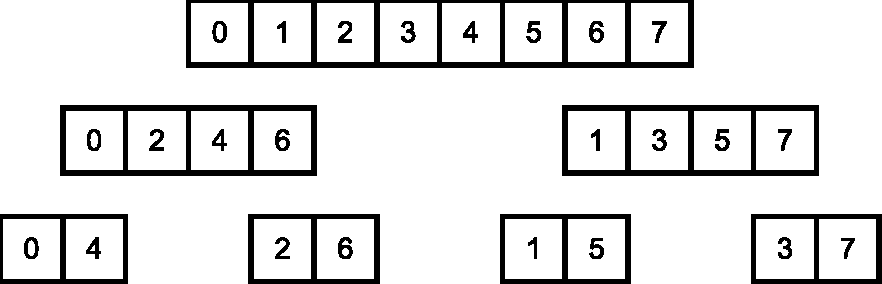
\includegraphics[scale=0.7]{assets/bit_reversal.pdf}
	\caption{Podział w kolejnych krokach rekurencyjnych}
	\label{fig:bit_reversal}
\end{figure}

\begin{lstfloat}[H]
\lstset{language=Python}
\begin{lstlisting}[frame=single]
def fft(input_arr):
    input_arr = reverse_array_with_bit_indices(input_arr)
    num_bits = int(np.ceil(np.log2(len(input_arr))))

    for step in range(1, num_bits+1):
        step_size = 1 << step
        omega = cmath.exp(-2j * math.pi / step_size)
        for start in range(0, len(input_arr), step_size):
            omega_power = 1
            for i in range(step_size // 2):
                index_even = start + i
                index_odd = start + i + step_size // 2
                temp = input_arr[index_even]
                input_arr[index_even] += (
                        omega_power * input_arr[index_odd])
                input_arr[index_odd] = (
                        temp - omega_power * input_arr[index_odd])
                omega_power *= omega

    return input_arr
\end{lstlisting}
\caption{Implementacja algorytmu Cooleya-Tukeya w języku Python}
\label{lst:fft_python}
\end{lstfloat}
\subsubsection{Testowe dane wejściowe}
Do poprawnego działania algorytmu Cooleya-Tukeya potrzebny jest wektor o długości $N = 2^n,$ gdzie $n \in \mathbb{N}$. W projekcie użyliśmy wektora liczb zespolonych, zawierającego liczby, których część rzeczywista jest losowana z przedziału 0 do 1,a część urojona jest równa 0. Oznacza to, że przypomina ona sygnał złożony z liczb rzeczywistych ale tablicę wejściową można modyfikować wynikami uzyskanymi w trakcie transformacji, które są liczbami zespolonymi.
\section{Przygotowanie środowiska}
Wszystkie testy oraz cała konfiguracja została wykonana na komputerze wyposażonym w 6-rdzeniowy, 12-wątkowy procesor AMD Ryzen 5 5600 z dostępem do 32 GB pamięci RAM.
Systemem operacyjnym zainstalowanym na komputerze jest Debian 12.
\subsection{Konfiguracja CMake}
W projekcie użyliśmy szeroko znanego narzędzia do zarządzania procesem kompilacji, programu "CMake". W przypadku programów sekwencyjnych oraz MPI nie skorzystaliśmy z CMake, ponieważ nie było takiej potrzeby.
Dla SYCL bardzo wygodnym i przydatnym narzędziem była funkcja \texttt{CMAKE\_EXPORT\_COMPILE\_COMMANDS} na potrzeby programu clangd. W tym przypadku narzędzia użyliśmy w większości dla zwiększenia wygody pracy. Bardzo podstawowym przykładem zawartości pliku konfiguracyjnego \emph{CMakeLists.txt} może być ten zawarty w listingu \ref{lst::cmake-SYCL}.

\begin{lstfloat}
\begin{lstlisting}[frame=single]
cmake_minimum_required(VERSION 3.0)

set(CMAKE_CXX_COMPILER "icpx")
set(CMAKE_CXX_FLAGS "${CMAKE_CXX_FLAGS}-fsycl -O3 -std=c++17")
set(CMAKE_EXPORT_COMPILE_COMMANDS ON)

project(FFT_SYCL LANGUAGES CXX)
set(SOURCES 
    src/main.cpp
)

add_executable(main ${SOURCES})
\end{lstlisting}
\caption{Plik konfiguracyjny CMakeLists.txt rozwiązań używających SYCL}
\label{lst::cmake-SYCL}
\end{lstfloat}

Biblioteka Distributed Ranges przysporzyła pewnych kłopotów. Na dzień w którym przygotowywaliśmy środowisko do użycia narzędzia, rozwiązanie z repozytorium projektu w serwisie GitHub nie działało poprawnie. Jako przykład wzięliśmy rozwiązanie z pobocznego repozytorium, zawierającego przykładowy projekt używający tej biblioteki \cite{dist-ranges-tutorial}.
\subsection{Użyte Kompilatory}
Kompilując programy implementujące sekwencyjne podejście do wybranych problemów użyliśmy Kolekcji Kompilatorów GNU (ang. \emph{GNU Compiler Collection}, GCC) dołączonej do systemu Debian.

Bardzo ważną częścią konfiguracji jest zestaw narzędzi oneAPI udostępniany przez firmę Intel. Pozostałe kompilatory użyte do obsługi MPI, SYCL a także Distributed Ranges pochodzą z tej właśnie kolekcji. Poradnik instalacji paczki dla systemów z grupy GNU/Linux znajduje się pod adresem \cite{oneapi-install}. Aby zapewnić poprawnie działanie przygotowanych w ramach projektu programów należy uruchomić skrypt ustawiający odpowiednie zmienne w powłoce. Domyślną ścieżką tego skryptu po instalacji zestawu oneAPI jest \emph{/opt/intel/oneapi/setvars.sh}.

Kompilatory użyte do poszczególnych narzędzi:
\begin{itemize}
\item Programy Sekwencyjne - \textbf{gcc/g++},
\item MPI - \textbf{mpicxx},
\item SYCL oraz Distributed Ranges - \textbf{icx/icpx}.
\end{itemize}

\subsection{Inne narzędzia}
Narzędziem, którego użyliśmy przy pisaniu implementacji niektórych algorytmów był program Scalasca \cite{scalasca}. Aplikacja służy do analizy przebiegu programów równoległych napisanych przy użyciu modeli MPI oraz Open-MP. Okazało się ono bardzo przydatne do wykrywania problemów z wydajnością dla moich implementacji w języku MPI.

Zachodzi potrzeba wspomnienia o pewnym niewygodnym, problemie który pojawił się przy próbie konfiguracji \emph{clangd}, serwera językowego usprawniającego pisanie kodu poprzez dodanie funkcjonalności do edytora tekstu takich jak uzupełnianie kodu czy szybki dostęp do definicji. Okazało się bowiem, iż zestaw oneAPI zawiera własną wersję tego narzędzia, znajduje się ona pod ścieżką \emph{/opt/intel/oneapi/compiler/latest/bin/compiler/clangd}. Niestety podana kompilacja nie wykrywała poprawnie plików nagłówkowych zawartych we własnym zestawie, co wymagało własnoręcznej kompilacji narzędzia z odpowiednim kompilatorem (\texttt{icpx}).

W katalogu głównym projektu zamieściliśmy skrypt \emph{build\_all.sh} służący do kompilacji wszystkich plików źródłowych i zapisania ich w katalogu \emph{build.}

\chapter{Problemy implementacyjne}
Podczas implementacji rozwiązań poszczególnych problemów, często pojawiały się specyficzne dla danego narzędzia problemy. Opisaliśmy je w podrozdziałach razem z dokładniejszym wytłumaczeniem działania oraz komentarzem na temat finalnych czasów wykonania każdego podejścia.
\section{Całkowanie metodą Monte Carlo}
Metoda Monte Carlo jest najłatwiejszą w implementacji częścią projektu. Wynika to z tego, że problem jest zawstydzająco równoległy. Jedyna komunikacja jaka zachodzi w przypadku rozwiązań równoległych, to końcowe zebranie danych do jednej zmiennej wątku głównego w celu obliczenia finalnego wyniku.
\subsection{Przegląd krytycznych części programu}
Bardzo ważną kwestią w przypadku metody Monte Carlo jest dobór odpowiedniego generatora liczb pseudolosowych. Do tego celu wykorzystaliśmy generator z biblioteki standardowej języka C++ \texttt{std::minstd\_rand.} Ten generator wybraliśmy ze względu na dostępność w każdym z użytych narzędzi. W przypadku modelu SYCL oraz biblioteki Distributed Ranges konieczne było użycie generatora z nagłówka \texttt{<oneapi/dpl/random>} o takiej samej nazwie (\texttt{oneapi::dpl::minstd\_rand}). Konfiguracja tych dwóch implementacji jest pokazana na listingach \ref{lst:minstd-rand} i \ref{lst:minst-rand-SYCL}.

\begin{lstfloat}
\lstset{language=C++}
\begin{lstlisting}[frame=single]
int a = -1, b = 1
std::random_device rd;
std::minstd_rand gen(rd());
std::uniform_real_distribution<double> dis(a, b);
\end{lstlisting}
\caption{Konfiguracja generatora \texttt{std::minstd\_rand.}}
\label{lst:minstd-rand}
\end{lstfloat}

\begin{lstfloat}
\lstset{language=C++}
\begin{lstlisting}[frame=single]
int a = -1, b = 1
//idx to numer obecnie wykonywanej iteracji petli glownej.
oneapi::dpl::minstd_rand gen(83734727, idx);
oneapi::dpl::uniform_real_distribution<double> dis(a, b);
\end{lstlisting}
\caption{Konfiguracja generatora \texttt{oneapi::dpl::minstd\_rand.}}
\label{lst:minst-rand-SYCL}
\end{lstfloat}

Poszczególne programy obliczają całkę funkcji
$$ f(x) = \sin{(\sum^n_{i=1}x_i^6)}; n=99 $$ gdzie $(x_1, x_2, \ldots, x_n)$ jest wektorem wejściowym.
Implementacja tej funkcji wygląda tak samo w każdym z programów. Można ją zobaczyć na listingu \ref{lst:calkowana-funkcja}.

\begin{lstfloat}
\lstset{language=C++}
\begin{lstlisting}[frame=single]
double f(std::vector<double> &x) {
  std::for_each(x.begin(), x.end(), [](double &val) {
    val = std::pow(val, 6);
  });
  return std::sin(std::reduce(x.begin(), x.end()));
}
\end{lstlisting}
\caption{Całkowana funkcja.}
\label{lst:calkowana-funkcja}
\end{lstfloat}

Główna pętla programu polega na wygenerowaniu punktu i zwiększaniu licznika w przypadku kiedy punkt znajduje się pod wykresem. Pokazaliśmy to na listingu \ref{lst:monte-carlo}.

\begin{lstfloat}
\lstset{language=C++}
\begin{lstlisting}[frame=single]
  int num_dimensions = 100, count_under = 0,
  	  num_iterations = 12 * 10000000,
      a = -1, b = 1;

  for (int i = 0; i < num_iterations; ++i) {
    std::for_each(x.begin(), x.end(),
      [&](double &val) { val = dis(gen); });
    count_under += f(x) > dis(gen);
  }
// typ __float128 pochodzi z pliku naglowkowego quadmath.h
  __float128 V = std::pow(b - a, num_dimensions);
  __float128 result = V * count_under / num_iterations;
\end{lstlisting}
\caption{Główna część programu całkującego metodą Monte Carlo.}
\label{lst:monte-carlo}
\end{lstfloat}

\subsection{Ostateczny czas wykonania - komentarz}
Pokazany na rysunku \ref{fig:wykonanie-MC} wykres przedstawia całkowity czas wykonania dla wszystkich wykonanych implementacji. Czas zmierzyliśmy przy użyciu narzędzia \texttt{/usr/bin/time} będącego zamiennikiem słowa kluczowego powłoki Bash \texttt{time.} \texttt{/usr/bin/time} daje większą ilość informacji, na przykład o liczbie błędów strony (ang. \emph{page fault}). Liczba wygenerowanych punktów wynosi $120000000.$

\begin{figure}
	\centering
	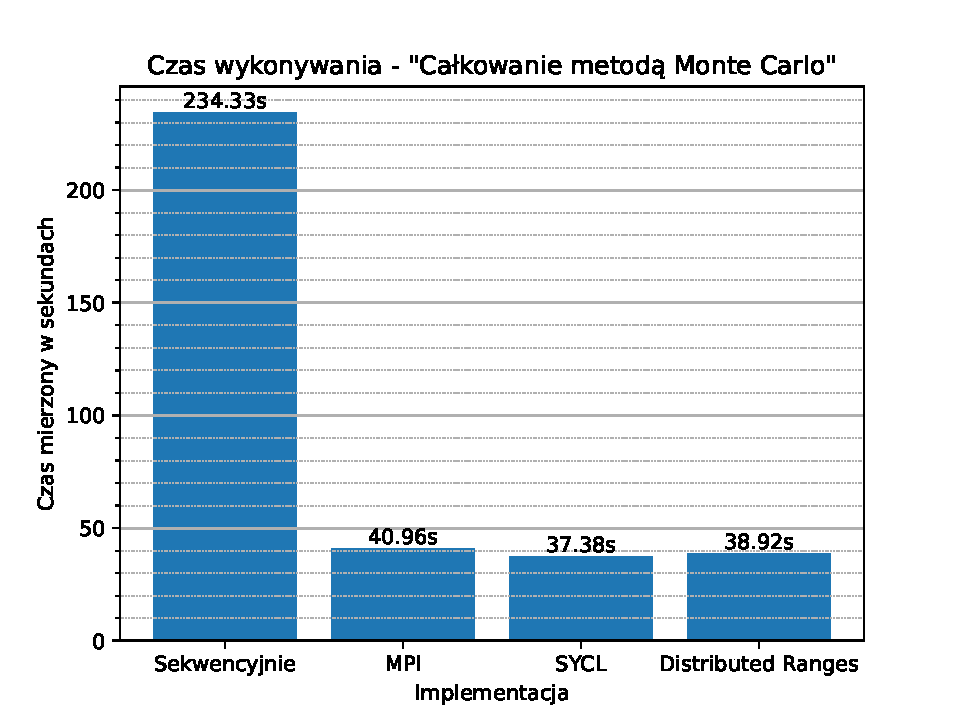
\includegraphics[scale=1]{assets/czas_wykonania_calkowanie.pdf}
	\caption{Wykres przedstawiający czas pracy różnych implementacji całkowania metodą Monte Carlo. Liczba wykorzystanych wątków dla programów równoległych wynosi 6.}
	\label{fig:wykonanie-MC}
\end{figure}

SYCL uzyskał najlepszy wynik z programów równoległych. Przyczyną tego jest wykorzystanie generatora liczb pseudolosowych z przestrzeni nazw \texttt{oneapi::dpl.} Przyspieszenie uzyskane przez narzędzia programowania równoległego w przypadku wykorzystania 6 wątków jest prawie sześciokrotne, czyli bliskie idealnemu.

\section{Metoda gradientu sprzężonego}
Metoda gradientu sprzężonego jest metodą iteracyjną w której obliczenia wykonywane w poszczególnych krokach są zależne od poprzedniego kroku. Ze względu na to, nie można nazwać problemu zawstydzająco równoległym. Przyspieszenie jest jednak możliwe do uzyskania poprzez równoleglizację operacji cząstkowych wykonywanych w ramach głównej pętli.

\subsection{Przegląd krytycznych części programu}
Funkcja zawierająca główną pętle programu jest bardzo podobna w każdej z implementacji. Kod pokazany na listingu \ref{lst:conjugate_gradient} przedstawia tę funkcję w jej sekwencyjnej wersji. Używając narzędzi SYCL, MPI oraz Distributed Ranges zrównoleglizowaliśmy kilka funkcji wykorzystanych w tej pętli.

\begin{lstfloat}
\lstset{language=C++}
\begin{lstlisting}[frame=single]
using vec = std::vector<double>;

vec conjugate_gradient(const vec &A, const vec &B) {
  double tolerance = 1.0e-27;

  uint32_t size = B.size();
  vec X(size, 0.0);

  vec residual = B;
  vec search_dir = residual;

  double old_resid_norm = norm(residual);

  while (old_resid_norm > tolerance) {
    vec A_search_dir = matrix_vector_multiply(A, search_dir);

    std::cout << old_resid_norm << '\n';

    double alpha = old_resid_norm * old_resid_norm /
                   inner_product(search_dir, A_search_dir);
    X = vector_combination(1.0, X, alpha, search_dir);
    residual = 
	  vector_combination(1.0, residual, -alpha, A_search_dir);

    double new_resid_norm = norm(residual);

    double pow = std::pow(new_resid_norm / old_resid_norm, 2);
    for (uint32_t i = 0; i < size; ++i) {
      search_dir[i] = residual[i] + pow * search_dir[i];
    }
    old_resid_norm = new_resid_norm;
  }

  return X;
}
\end{lstlisting}
\caption{Główna funkcja programu metody CG.}
\label{lst:conjugate_gradient}
\end{lstfloat}

\begin{itemize}
\item \texttt{vector\_combination} to funkcja przeprowadzająca kombinację liniową dwóch wektorów. Równoleglizowana jest poprzez podział wektora na kilka części i wykonanie pracy przez poszczególne wątki. W większości przypadków jest to przeprowadzane automatyczie przez wykorzystane narzędzie. Przykład takiego zachowania widać na Listingu \ref{lst:vector-combination}, gdzie pokazana jest implementacja tej funkcji w SYCL.
\item \texttt{inner\_product} wykonuje iloczyn skalarny dwóch wektorów. Do tego problemu są dwa podejścia. W przypadku SYCL, każdy wątek może dodawać wyniki mnożenia do wspólnej zmiennej. MPI oraz Distributed Ranges wymagają jednak wykonania dodatkowo operacji redukcji (ang. \emph{reduce}). Jest to zobrazowane we fragmencie kodu z implementacji z użyciem biblioteki Distributed Ranges zawartego na listingu \ref{lst:inner-product}.
\item \texttt{norm} to funkcja obliczająca normę euklidesową wektora. $$||x||_2 = \sqrt{\sum_{i=1}^Nx^2_i}, x = (x_1,x_2,\cdots,x_N) \in \mathbb{R}^N$$
\item \texttt{matrix\_vector\_multiply} ma za zadanie przemnożenie macierzy przez wektor dając nowy wektor wynikowy. Wykonywanie tej funkcji zajmuje programowi najwięcej czasu, więc jest ona punktem krytycznym. 
\end{itemize}

\begin{lstfloat}
\lstset{language=C++}
\begin{lstlisting}[frame=single]
void vector_combination(sycl::queue &queue, 
		sycl::buffer<double, 1> &vec1_buf,
        double mult, sycl::buffer<double, 1> &vec2_buf,
        int size) {
  queue.submit([&](sycl::handler &h) {
    auto vec1 = vec1_buf
    				.get_access<sycl::access::mode::read_write>(h);
    auto vec2 = vec2_buf.get_access<sycl::access::mode::read>(h);

    h.parallel_for(sycl::range<1>(size),
                   [=](sycl::id<1> i) { vec1[i] += vec2[i] * mult; });
  });
  queue.wait();
}
\end{lstlisting}
\caption{Funkcja \texttt{vector\_combination} z implementacji CG w SYCL.}
\label{lst:vector-combination}
\end{lstfloat}

\begin{lstfloat}
\lstset{language=C++}
\begin{lstlisting}[frame=single]
template <dr::distributed_range X>
double inner_product(X &&x, std::vector<double> &y) {
  auto zipped =
      dr::mhp::views::zip(x, y) | 
      dr::mhp::views::transform([](auto &&elem) {
        auto &&[a, b] = elem;
        return a * b;
      });

  return mhp::reduce(zipped);
}
\end{lstlisting}
\caption{Funkcja \texttt{inner\_product} z implementacji CG z użyciem Distributed Ranges.}
\label{lst:inner-product}
\end{lstfloat}

Implementacja algorytmu przy pomocy narzędzia SYCL była bardzo łatwa i intuicyjna, operacje nie różniły się bardzo od tych które wykonano w przypadku sekwencyjnym. 

Stworzenie działającego programu w MPI wymagało większych przygotowań i przemyślenia podejmowanych działań. Ważnym punktem rozważań było odpowiednie zarządzanie pamięcią pomiędzy procesami. W przygotowanym kodzie dane pobierane z pliku od razu dzielone są na równe części, aby nie zwiększać czasu poprzez komunikację. Jedyną tablicą, która jest przechowywana w całości w każdym z procesów jest zmienna \texttt{search\_dir.} Jest tak dlatego, że w każdym z kroków macierz $A$, która jest podzielona tak, aby każdy proces miał kilka z jej wierszy, jest mnożona przez ten wektor.

Największym problemem była operacja mnożenia macierzy przez wektor z wykorzystaniem biblioteki Distributed Ranges. O ile przestrzeń nazw \texttt{shp} posiada gotową implementacje dla tej operacji, \texttt{mhp} jest w tym zakresie o wiele bardziej uboga. Do implementacji zaszła potrzeba wykorzystania segmentów macierzy udostępnianych przez strukturę \texttt{dr::mhp::distributed\_vector.} W tym wypadku kod przypomina ten z implementacji MPI i spełnia jeden warunek, wielkość macierzy musi być podzielna przez liczbę użytych procesów. Ten fragment kodu pokazaliśmy w Listingu \ref{lst:dist-ranges-mat-vec}.

\begin{lstfloat}
\lstset{language=C++}
\begin{lstlisting}[frame=single]
template <dr::distributed_range X, dr::distributed_range Y>
void matrix_vector_multiply(X &&mat, std::vector<double> &vec, 
						   Y &&result,int size) {
  if (mhp::rank() == 0) {
    std::cout << "b\n";
  }

  auto segment = mat.segments()[mhp::rank()];
  int rows_in_segment = size / mhp::nprocs();
  std::vector<double> result_vec(rows_in_segment, 0);
  for (int i = 0; i < rows_in_segment; ++i) {
    for (int j=0; j < size; ++j) {
      result_vec[i] += segment[size * i + j] * vec[j];
    }
  }

  segment = result.segments()[mhp::rank()];
  for (int i = 0; i < rows_in_segment; ++i) {
    segment[i] = result_vec[i];
  }

  if (mhp::rank() == 0) {
    std::cout << "e\n";
  }

  mhp::barrier();
}

\end{lstlisting}
\caption{Funkcja \texttt{matrix\_vector\_multiply} z implementacji CG z użyciem Distributed Ranges.}
\label{lst:dist-ranges-mat-vec}
\end{lstfloat}

\subsection{Ostateczny czas wykonania - komentarz}
Rysunek \ref{fig:wykonanie-cg} pokazuje czas wykonania operacji z użyciem różnych narzędzi. Czas był mierzony dla dziesięciu wykonań metody gradientu sprzężonego, gdzie macierz wejściowa ma długość i szerokość mierzącą $1296000000$ elementów. Jak łatwo zauważyć, biblioteka Distributed Ranges wypadła najgorzej, proces przebiegał wolniej nawet niż w implementacji sekwencyjnej. Analizując problem dało się odkryć, że ogromną ilość czasu zajmuje mnożenie macierzy przez wektor. Niestety pomimo starań nie udało się doprowadzić tej implementacji do prędkości porównywalnych z SYCL oraz MPI. Można domyślać się, że ten efekt jest wywołany próbami komunikacji pomimo odwoływania się do pamięci, która powinna być rozpoznana jako lokalna. W dodatku, przyspieszenie uzyskane dla SYCL oraz MPI nie jest duże.

\begin{figure}
	\centering
	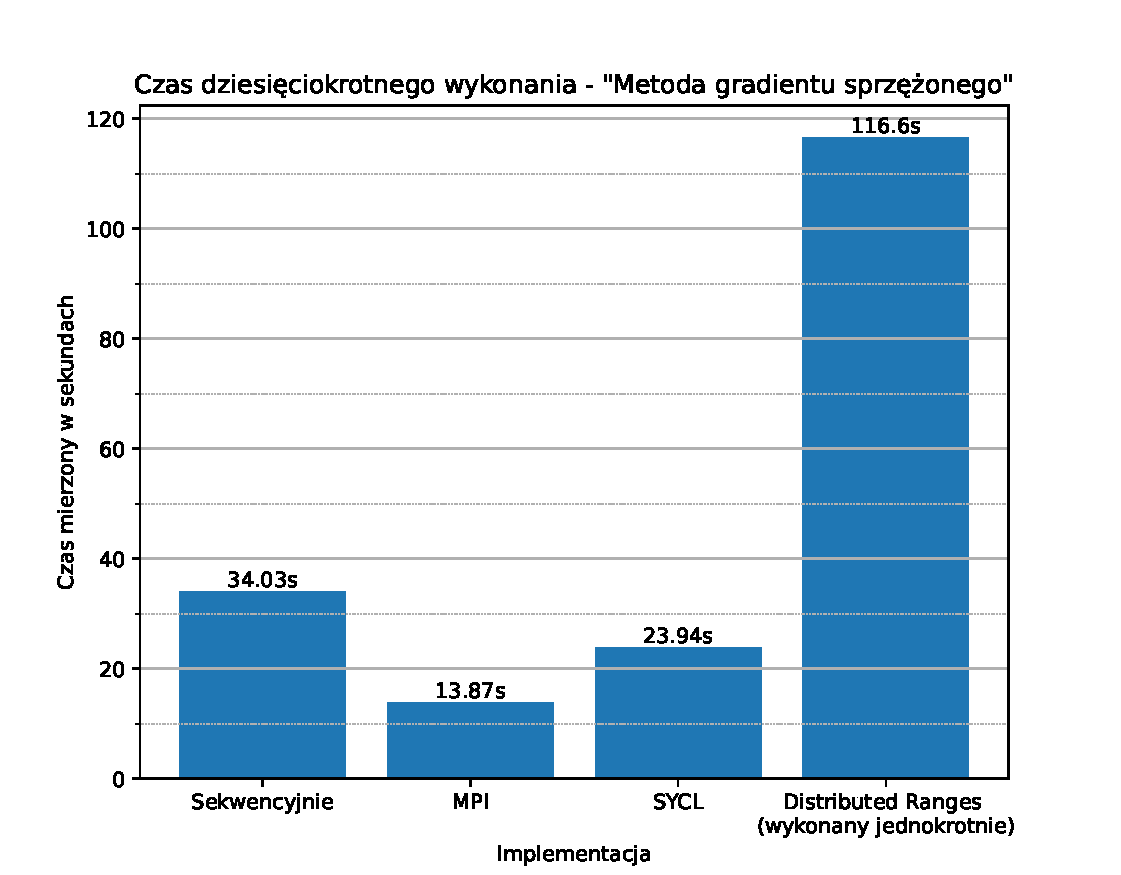
\includegraphics[scale=0.8]{assets/czas_wykonania_cg.pdf}
	\caption{Wykres przedstawiający czas pracy różnych implementacji metody gradientu sprzężonego. Liczba wykorzystanych wątków dla programów równoległych wynosi 6.}
	\label{fig:wykonanie-cg}
\end{figure}

\section{Szybka transformacja Fouriera}
Implementacja FFT okazała się najtrudniejszym problemem do
rozwiązania. Warunkiem poprawnego działania algorytmu jest rozmiar wektora wejściowego będący potęgą liczby 2. Ze względu na potrzebę uruchomienia programu na komputerze z procesorem sześciordzeniowym, to ograniczenie rozmiarowe powodowało problemy przy podziale danych. Potrzeba operowania na zbiorze danych z indeksami odwróconymi bitowo także była czynnikiem, który wymagał ostrożności przy implementacji.
\subsection{Przegląd krytycznych części programu}
Po wczytaniu danych z pliku, indeksy tablicy liczb wygenerowanej przez osobny program muszą zostać odwrócone bitowo. O ile program sekwencyjny nie jest trudny w wykonaniu, co widać na Listingu \ref{lst:bit-reverse-seq}, problem jest nietrywialny kiedy chcemy użyć pamięci rozproszonej. Ze względu na skończoną ilość pamięci operacyjnej komputera i dużą ilość danych do przetworzenia, konieczne byłoby tutaj użycie wyspecjalizowanego algorytmu stworzonego do tego działania. Przez wysoki poziom trudności utworzenia programu realizującego takie rozwiązanie, oraz porównywalnie małą ilość czasu zajmowaną przez tę operację, program napisany z użyciem modelu MPI korzysta z funkcji wprowadzonych w MPI-3 \cite{mpi41}. Problem ten rozwiązaliśmy w sposób pokazany na listingu \ref{lst:bit-reverse-mpi}.

\begin{lstfloat}
\lstset{language=C++}
\begin{lstlisting}[frame=single]
void bit_reverse_indices(size_t size, unsigned long num_bits,
                         Complex *input_array) {
  Complex *temp_array = new Complex[size];
  std::copy(input_array, input_array + size, temp_array);
  unsigned long tableSize = 1 << num_bits;
  for (unsigned long i = 0; i < tableSize; ++i) {
    unsigned long reversed = 0;
    for (unsigned long j = 0; j < num_bits; ++j) {
      if (i & (1 << j)) {
        reversed |= (1 << (num_bits - 1 - j));
      }
    }
    input_array[i] = temp_array[reversed];
  }
}
\end{lstlisting}
\caption{Implementacja sekwencyjna operacji odwrócenia bitowego indeksów tabeli liczb zespolonych.}
\label{lst:bit-reverse-seq}
\end{lstfloat}

\begin{lstfloat}
\lstset{language=C++}
\begin{lstlisting}[frame=single]
void bit_reverse_indices(MPI_Win &win, Complex *global_array,
 						int size, int rank, int root,
 						int num_procs, int num_bits) {
  int *sendcnts = new int[num_procs];
  int *displs = new int[num_procs];

  for (int i = 0; i < num_procs - 1; ++i) {
    sendcnts[i] = size / num_procs;
    displs[i] = i * (size / num_procs);
  }
  sendcnts[num_procs - 1] = (size / num_procs) + size % num_procs;
  displs[num_procs - 1] = (num_procs - 1) * (size / num_procs);

  Complex *local_array = new Complex[sendcnts[rank]];

  MPI_Scatterv(global_array, sendcnts, displs,
  			  MPI_DOUBLE_COMPLEX, local_array, sendcnts[rank],
  			  MPI_DOUBLE_COMPLEX, 0, MPI_COMM_WORLD);

  MPI_Win_lock(MPI_LOCK_SHARED, rank, MPI_MODE_NOCHECK, win);
  for (int i = 0; i < sendcnts[rank]; ++i) {
    global_array[reverse_bits(i + displs[rank], num_bits)] 
    	  = local_array[i];
  }
  MPI_Win_unlock(rank, win);

  delete[] local_array;
  delete[] sendcnts;
  delete[] displs;

  MPI_Barrier(MPI_COMM_WORLD);
}
\end{lstlisting}
\caption{Implementacja z użyciem MPI operacji odwrócenia bitowego indeksów tabeli liczb zespolonych.}
\label{lst:bit-reverse-mpi}
\end{lstfloat}

Główna pętla programu sekwencyjnego wygląda tak jak na listingu \ref{lst:fft-seq}. Ważnym zabiegiem, który trzeba było zastosować aby program był wykonywany szybko, jest sekwencyjne liczenie potęgi liczby przechowywanej w zmiennej \texttt{omega}. Bez tego, wysokie potęgi tej liczby musiałyby być liczone przy każdej operacji wykonywanej przez program. Co ciekawe, kompilator SYCL poprawia naiwne liczenie tych potęg automatycznie, zachowując odpowiednią wydajność.

\begin{lstfloat}
\lstset{language=C++}
\begin{lstlisting}[frame=single]
void fft(Complex *input_array, int size) {
  size_t num_bits = std::log2(size);
  bit_reverse_indices(size, num_bits, input_array);

  for (int i = 1; i <= num_bits; ++i) {
    int step_size = 1 << i;
    Complex omega = std::exp(-2.0 * J * M_PI / (double) step_size);

    for (int start = 0; start < size; start += step_size) {
      Complex omega_power = 1;
      for (int j = 0; j < step_size / 2; j++) {
        int index_even = start + j;
        int index_odd = start + j + step_size / 2;
        Complex temp = input_array[index_even];
        input_array[index_even] += 
        	  omega_power * input_array[index_odd];
        input_array[index_odd] = 
          temp - omega_power * input_array[index_odd];
        omega_power *= omega;
      }
    }
  }
}

\end{lstlisting}
\caption{Implementacja pętli głównej algorytmu szybkiej transformacji Fouriera.}
\label{lst:fft-seq}
\end{lstfloat}

Zarówno w przypadku MPI jak i SYCL, ważną optymalizacją był podział problemu na dwa przypadki zależne od wielkości pojedynczego kroku. Należy zauważyć, że w przypadku gdy zmienna \texttt{step\_size} zawiera wartości bardzo małe, lepszym rozwiązaniem jest zrównoleglenie pętli wewnętrznej, czyli wykonywanie kilku kroków na raz aby ograniczyć komunikację między wątkami. W przypadku odwrotnym nie byłoby wystarczająco wiele kroków aby podzielić je na kilkanaście wątków, ale każdy krok operuje na ilości danych na tyle dużej, że komunikacja nie jest problemem. Implementacja z użyciem MPI ma dodatkowy powód na zastosowanie takiego zabiegu. Podział danych utworzony na początku wymaga, aby ilość danych przychowywanych w lokalnie dla jednego wątku była podzielna przez rozmiar kroku. Jeżeli ten warunek nie zostanie zachowany, to obliczenia nie zostaną wykonane poprawnie.

W przypadku MPI, podział danych pokazany na listingu \ref{lst:mpi-data-split} jest wystarczający do momentu gdy lokalny dla wątku rozmiar danych jest podzielny przez rozmiar kroku. W sytuacji gdy rozmiar kroku przekracza tę wartość, potrzebny jest nowy podział. Rozwiązanie zastosowane w tej implementacji jest proste. Dla każdego kroku następuje podział danych na tablicę przechowującą wartości o indeksach  parzystych oraz drugą z indeksami nieparzystymi. Obliczenia wykonywane są jak dotychczas i dane zwracane są do jednego wątku aby można było powtórzyć proces. Listing \ref{lst:mpi-data-split2} zawiera kod dokonujący tego podziału. Niestety, taka operacja wymaga dużej ilości komunikacji pomiędzy wątkami, co odbije się znacznie na ostatecznym wyniku.

\begin{lstfloat}
\lstset{language=C++}
\begin{lstlisting}[frame=single]
  int *sendcnts = new int[num_procs]();
  int *displs = new int[num_procs]();
  int *displs_odd = new int[num_procs]();
  for (int i = 0; i < num_procs; ++i) {
    sendcnts[i] = 0;
    displs[i] = 0;
  }
  int closest_pow_2_num_procs = 1;
  while (closest_pow_2_num_procs < num_procs) {
    closest_pow_2_num_procs zu<<= 1;
  }
  int base_num = size / closest_pow_2_num_procs;
  int additional =
      (size - base_num * num_procs) / (closest_pow_2_num_procs >> 1);

  for (int i = 0; i < num_procs; ++i) {
    sendcnts[i] = base_num;
    if (i < (closest_pow_2_num_procs >> 1)) {
      sendcnts[i] += additional;
    }
    for (int j = i + 1; j < num_procs; ++j) {
      displs[j] += sendcnts[i];
    }
  }

  std::vector<Complex> local_array(sendcnts[rank]);

  MPI_Scatterv(global_array, sendcnts, displs, MPI_DOUBLE_COMPLEX,
               local_array.data(), sendcnts[rank],
               MPI_DOUBLE_COMPLEX, root, MPI_COMM_WORLD);
\end{lstlisting}
\caption{Pierwszy podział danych potrzebny do wykonania szybkiej transformacji Fouriera w MPI.}
\label{lst:mpi-data-split}
\end{lstfloat}

\begin{lstfloat}
\lstset{language=C++}
\begin{lstlisting}[frame=single]
for (int start = 0; start < size; start += step_size) {
  // Dla kazdego kroku podzial danych.
  base_num = step_size / 2 / num_procs;
  additional = (step_size / 2) - base_num * num_procs;
  for (int j = 0; j < num_procs - 1; ++j) {
    sendcnts[j] = base_num;
    displs[j] = j * base_num + start;
    displs_odd[j] = j * base_num + start + (step_size / 2);
  }
  endcnts[num_procs - 1] = base_num + additional;
  displs[num_procs - 1] = (num_procs - 2) * base_num + start;
  displs_odd[num_procs - 1] =
    (num_procs - 2) * base_num + start + (step_size / 2);

  MPI_Scatterv(global_array, sendcnts, displs, MPI_DOUBLE_COMPLEX,
               local_array.data(), sendcnts[rank], 
               MPI_DOUBLE_COMPLEX, root, MPI_COMM_WORLD);
  MPI_Scatterv(global_array, sendcnts, displs_odd, 
  			   MPI_DOUBLE_COMPLEX, local_array_odd.data(),
  			   sendcnts[rank], MPI_DOUBLE_COMPLEX,
               root, MPI_COMM_WORLD);
  //WYKONANIE OBLICZEN
  MPI_Gatherv(local_array.data(), sendcnts[rank], MPI_DOUBLE_COMPLEX,
              global_array, sendcnts, displs, 
              MPI_DOUBLE_COMPLEX, root, MPI_COMM_WORLD);
  MPI_Gatherv(local_array_odd.data(), sendcnts[rank], 
  			  MPI_DOUBLE_COMPLEX, global_array, sendcnts, 
  			  displs_odd, MPI_DOUBLE_COMPLEX, root, MPI_COMM_WORLD);
}

\end{lstlisting}
\caption{Drugi podział danych potrzebny do wykonania szybkiej transformacji Fouriera w MPI.}
\label{lst:mpi-data-split2}
\end{lstfloat}

Przez brak odpowiednich narzędzi do zarządzania podziałem pamięci w strukturach oferowanych przez bibliotekę Distributed Ranges implementacja FFT przy użyciu tego narzędzia okazała się niemożliwa. Korzystając z tej biblioteki można równocześnie używać funkcji z MPI, lecz w takim wypadku utrudniłoby to niepotrzebnie pracę.

Ostatnią rzeczą, o której warto wspomnieć jest zużycie pamięci. Pomimo, że nie ma ono wpływu na długość działania programu, to implementacja MPI korzysta z dwukrotnie większej ilości pamięci operacyjnej ze względu na konieczność podziału na podzadania z jednoczesnym utrzymaniem całego zbioru danych w jednym z procesów.

\subsection{Ostateczny czas wykonania - komentarz}
Na rysunku \ref{fig:wykonanie-fft} widać, że implementacja z użyciem modelu MPI dała o wiele lepszy wynik niż implementacja SYCL, nawet pomimo dużej potrzeby komunikacji w końcowej fazie wykonywania algorytmu. Pomimo to, napisanie tego programu używając SYCL było o wiele łatwiejsze i zajęło dużo mniej czasu.

\begin{figure}
	\centering
	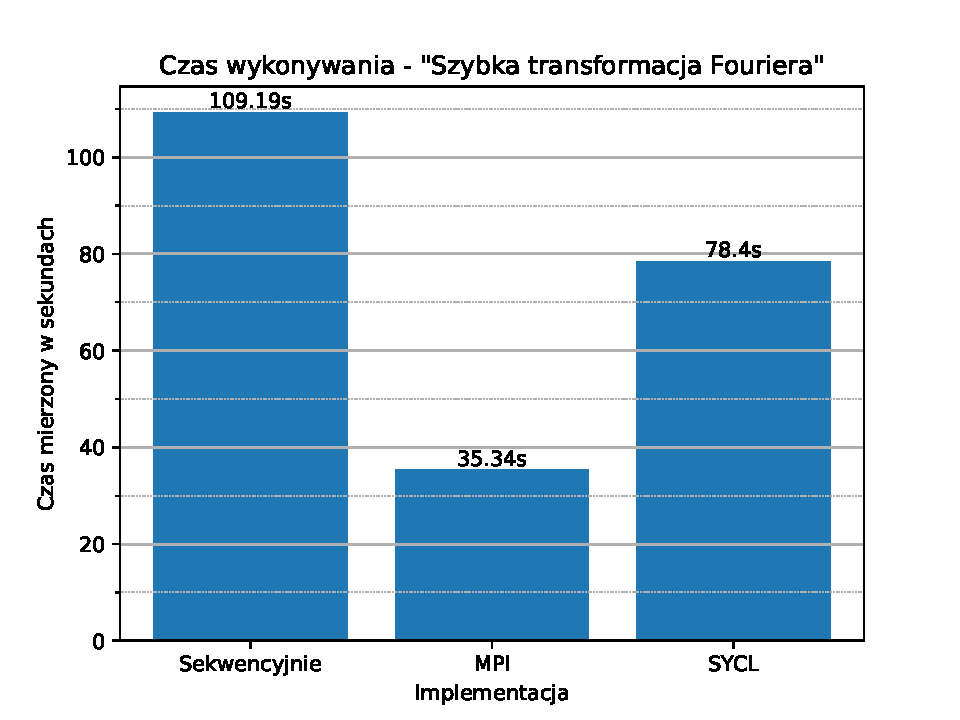
\includegraphics[scale=0.8]{assets/czas_wykonania_fft.pdf}
	\caption{Wykres przedstawiający czas pracy różnych implementacji szybkiej transformaty Fouriera. Liczba wykorzystanych wątków dla programów równoległych wynosi 6.}
	\label{fig:wykonanie-fft}
\end{figure}

\chapter{Porównanie łatwości w użyciu}
W tym rozdziale zawarliśmy subiektywną opinię opisaną z perspektywy osoby, która po raz pierwszy używała każdego z opisanych narzędzi. Kwestia wydajności poszczególnych rozwiązań jest pomijana i skupiliśmy się jedynie na łatwości w użyciu.

Implementacja równoległych rozwiązań w MPI okazała się najtrudniejsza, co jest wynikiem przewidywalnym. MPI daje pełną kontrolę nad podziałem pamięci i nad sposobem komunikacji pomiędzy poszczególnymi procesami. Przez to łatwo jest popełnić drobne, trudne do znalezienia błędy związane z zarządzaniem tymi elementami programu. Liczba napisanych linijek kodu jest o wiele większa od pozostałych rozwiązań. Model MPI wymaga dobrego zrozumienia oraz dużej wiedzy na temat poprawnych praktyk aby pisać kod dobrej jakości, który w dodatku jest wydajny.

Pisanie kodu w SYCL jest w porównaniu do MPI przyjemne i szybkie. Model wymagał jednak pewnego rodzaju początkowego obeznania, gdyż wprowadza wiele specyficznych metod tworzenia oprogramowania, które nie są od początku intuicyjne. Jako dobre wprowadzenie do SYCL można polecić książkę \cite{sycl-book}, która bardzo dobrze wyjaśnia zarówno podstawowe techniki, jak i te bardziej zaawansowane. Narzędzie było na tyle wygodne, że wykorzystano je przy tworzeniu programów do generacji danych wejściowych zarówno dla metody gradientu sprzężonego jak i szybkiej transformaty Fouriera.

Distributed Ranges po raz kolejny jest trudnym przypadkiem do opisania, braki w funkcjonalnościach przestrzeni nazw \emph{mhp} uniemożliwiają, efektywne wprowadzenie biblioteki do jakiegokolwiek większego projektu. Jeżeli chcemy użyć struktur danych zawartych w bibliotece, wymuszony zostaje rodzaj pracy podobny do tego w MPI, lecz bardziej ograniczony, co widać w implementacji metody gradientu sprzężonego. Narzędzie, pomimo wad ma jednak duży potencjał. Funkcje, które są obecnie zaimplementowane są bardzo intuicyjne w użyciu. Praca ze strukturami prawie nie różni się od pracy z biblioteką \emph{<ranges>} ze standardu C++20. Wynikającym z równoległej natury biblioteki problemem jest brak możliwości przekazywania referencji do wyrażeń lambda używanych w pracy z widokami, co w przypadku \emph{<ranges>} jest bardzo użyteczne. Podobne zachowanie można zaobserwować w SYCL, który jest eksploatowany przez Distributed Ranges. Ciekawe jest, w jaki sposób narzędzie będzie się rozwijało dalej. Za naturalną ścieżkę rozwoju możnaby uznać przeniesienie funkcjonalności z przestrzeni \emph{shp,} takich jak funkcji mnożenia macierzy przez wektor, do części \emph{mhp.}

\chapter{Porównanie wydajności}
Wyniki badania wydajności metody Monte Carlo są pokazane na rysunku \ref{fig:monte-carlo-speedup}. Wykres ten pokazuje przyspieszenie w zależności od ilości wątków. Każdy z programów był kompilowany z użyciem flagi \emph{"-O1"} po to, aby kompilator nie używał automatycznej wektoryzacji. Jak widać na wykresie, różnice pomiędzy przyspieszeniem uzyskanym dla poszczególnych implementacji są niewielkie. Niewielką przewagę nad pozostałymi uzyskał SYCL, szczególnie dobrze zdaje się on radzić sobie z wykorzystaniem wielowątkowości współbieżnej często dostępnej w nowoczesnych procesorach. Odwrotną sytuację widzimy w przypadku biblioteki Distributed Ranges. Dla tego rozwiązania przyspieszenie uzyskane dla 6 wątków, nie różni się w istotny sposób przpadku z 12 użytymi wątkami.

\begin{figure}
	\centering
	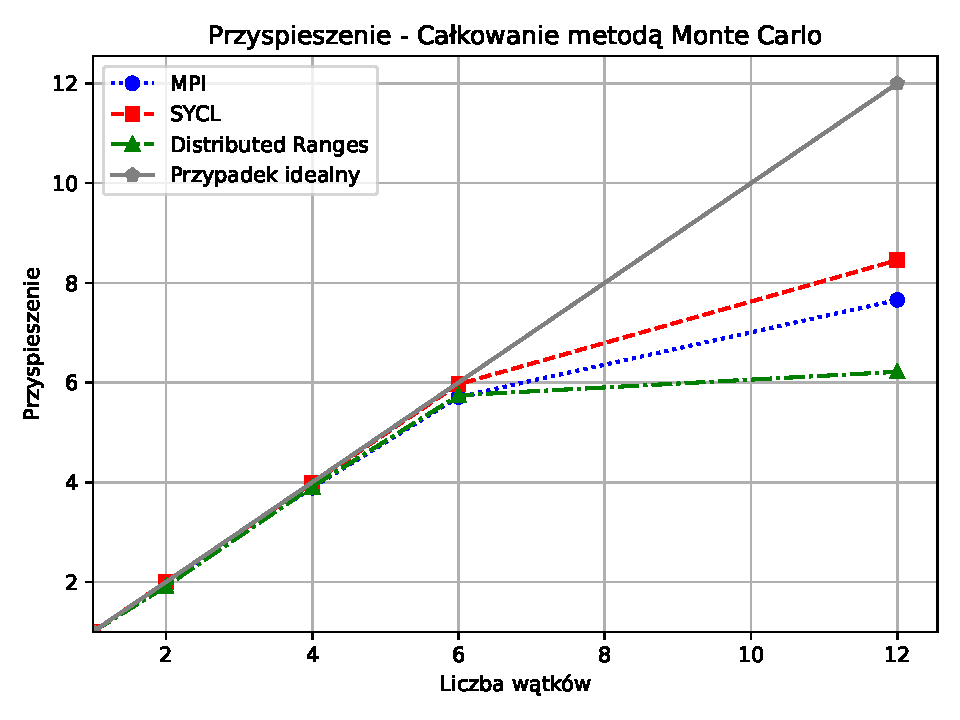
\includegraphics[scale=1]{assets/przyspieszenie_calkowanie.pdf}
	\caption{Przyspieszenie całkowania metodą Monte Carlo w zależności od ilości wykorzystanych wątków.}
	\label{fig:monte-carlo-speedup}
\end{figure}

Metoda CG uzyskała niewielkie przyspieszenie pokazane na rysunku \ref{fig:cg-speedup}. W przypadku uruchomienia programu MPI z użyciem jednego wątku wynik wyglądał gorzej, niż ten uzyskany przez implementację sekwencyjną. Poprawił się do poziomu ponad dwukrotnego przyspieszenie przy użyciu czterech wątków jednak później zaczął spadać. SYCL spisał się jeszcze gorzej, uzyskując prawidłowe przyspieszenie dla 2 wątków i schodząc coraz niżej wraz ze wzrostem ich liczby. Metoda gradientu sprzężonego jest w głównej swojej części metodą sekwencyjną. Nie można było się spodziewać dużej zmiany. Być może wynik mógłby zostać poprawiony poprzez użycie wektoryzacji operacji podczas mnożenia macierzy przez wektor lub zastosowanie wersji algorytmu która jest stworzona do zrównoleglania.

\begin{figure}
	\centering
	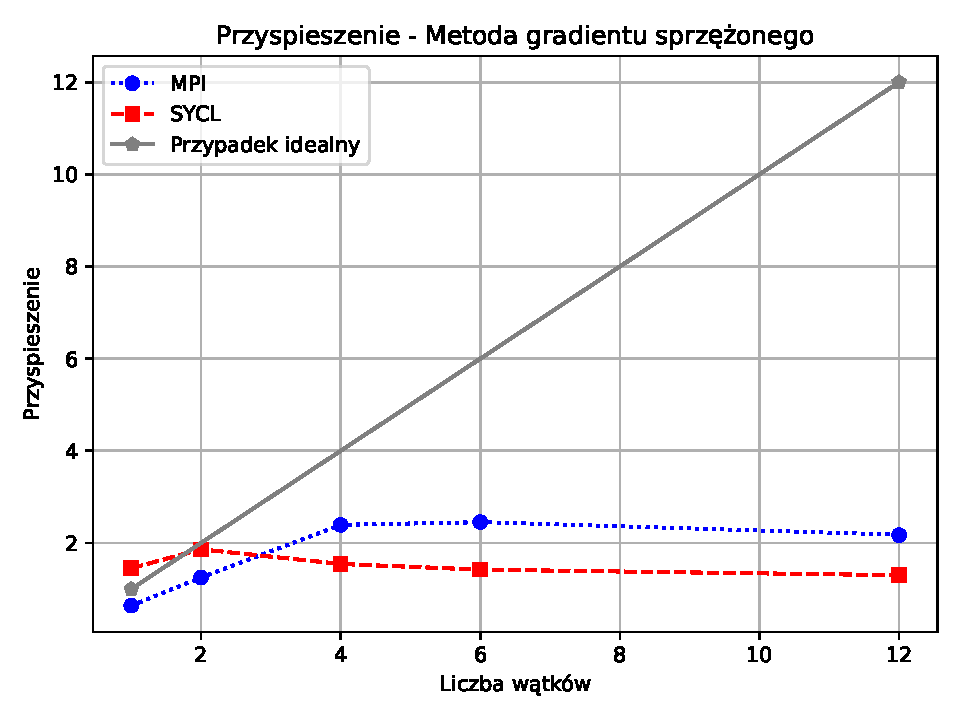
\includegraphics[scale=1]{assets/przyspieszenie_cg.pdf}
	\caption{Przyspieszenie metody gradientu sprzężonego w zależności od ilości wykorzystanych wątków.}
	\label{fig:cg-speedup}
\end{figure}

Rysunek \ref{fig:fft-speedup} obrazuje wyniki testów implementacji szybkiej transformacji Fouriera. Ze względu na błędy obliczeniowe powstałe przy uruchamianiu programu z użyciem mniej niż czterech wątków, linia na wykresie reprezentująca MPI jest skrócona. Przyspieszenie obliczyliśmy względem wyniku uzyskanego przez program sekwencyjny. Obie implementacje uzyskały drobne przyspieszenie. W przypadku MPI, program uzyskał bardzo dobry wynik dla czterech wątków. Złożyło się na to kilka czynników. Cztery jest potęgą liczby dwa co bardzo upraszcza podział danych. Ponadto, przez zmniejszenie liczby wątków zmniejsza się wymagana ilość komunikacji między wątkami. To wszystko składa się na wynik widoczny na wykresie. Słaby poziom uzyskany przez SYCL jest zapewne efektem naiwnej implementacji, która może zostać usprawniona użyciem innej wersji algorytmu lub lepszym zarządzaniem danymi.

\begin{figure}
	\centering
	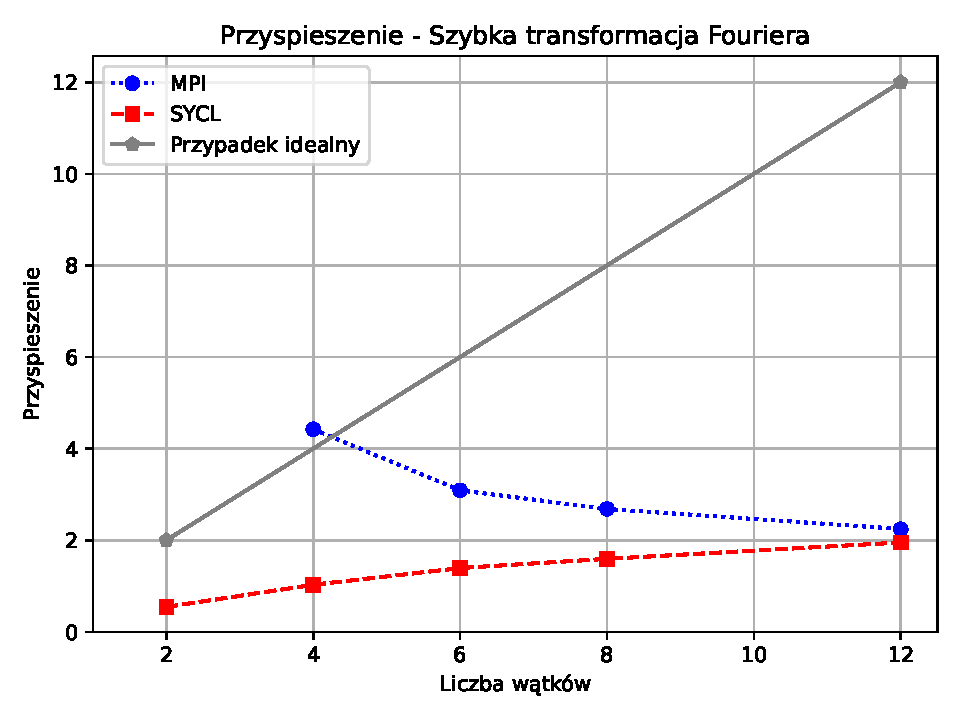
\includegraphics[scale=1]{assets/przyspieszenie_fft.pdf}
	\caption{Przyspieszenie szybkiej transformacji Fouriera w zależności od ilości wykorzystanych wątków.}
	\label{fig:fft-speedup}
\end{figure}

\section{Wnioski}
Programowanie równoległe jest bardzo trudną sztuką wymagającą dobrego panowania nad zasobami komputera. Przedstawione wyniki potwierdzają, że o ile łatwe problemy można rozwiązać w stosunkowo prosty sposób używając każdego z wymienionych narzędzi, to bardziej skomplikowane algorytmy wymagają od nas kontroli nawet korzystając z opcji mających na celu ułatwienie tego procesu. Pomimo włożonych starań, biblioteka Distributed Ranges była użyteczna tylko w przypadku całkowania metodą Monte Carlo którą można uznać za problem trywialny. Przy zadaniach o większym poziomie trudności niekompletność narzędzia była blokadą nie do przejścia. MPI wypadł w tym zestawieniu wydajności korzystnie na tle konkurentów, jednak to SYCL był najłatwiejszy w użyciu. Pewnym jest, że przedstawione implementacje mogą być przekształcone w bardziej wydajne i da się uzyskać wynik lepszy od tego otrzymanego w tym projekcie. Jeden rok nie jest wystarczającym czasem aby poznać wszystkie tajniki tych bogatych w funkcjonalności modeli. 


\chapter*{Podsumowanie}
\addcontentsline{toc}{chapter}{Podsumowanie}
Patrząc na wyniki testów można wyciągnąć kilka wniosków. Każde z przedstawionych narzędzi ma swoje konkretne zastosowanie. MPI jest od wielu lat standardem w programowaniu systemów wykorzystujących pamięć rozproszoną. Spośród opisanych w pracy, ten model jest także najbardziej wydajny ponieważ daje użytkownikowi największą kontrolę nad zasobami komputera. Niestety, wysokie możliwości przychodzą kosztem konieczności zdobycia dużej wiedzy oraz obycia aby wykorzystać to narzędzie poprawnie. Odpowiedzią na ten problem jest SYCL. To narzędzie, mimo, że nie jest wstanie operować pamięcią rozproszoną, dość wydajnie radzi sobie z programowaniem równoległym korzystając z pamięci wspólnej. Ta warstwa abstrakcji pozostaje przy tym bardzo wygodna i łatwa w użyciu, zapewniając proste w użyciu funkcje umożliwiające wysoce produktywną pracę. Distributed Ranges, pomimo oczywistej potrzeby rozwoju oraz wprowadzenia wielu poprawek, jest narzędziem które oferuje szybki dostęp do operacji równoległych za pośrednictwem SYCL w przestrzeni nazw \emph{shp}. Niestety, jak widać w wynikach testów, część wykorzystująca MPI nie jest jeszcze gotowa do eksploatacji w większej skali. Wiele kluczowych funkcji nie jest zaimplementowane, a te, które istnieją, potrafią być problematyczne. Jednak jeżeli \emph{mph} nadal będzie rozwijana, to ma potencjał na połączenie możliwości programowania z pamięcią rozproszoną znanej z MPI oraz łatwości i produktywności jaką oferuje SYCL oraz biblioteka \emph{<ranges>} z C++20. Aby jeszcze dokładniej określić zależności między przedstawionymi narzędziami, odpowiednim krokiem byłaby implementacja rozwiązań kolejnych problemów bądź użycie wyspecjalizowanych algorytmów do rozwiązania tych opisanych w tej pracy.


\listof{lstfloat}{Spis listingów} % jeśli są listingi
\addcontentsline{toc}{chapter}{Spis listingów}

\listoftables{} % jeśli są tabele
\addcontentsline{toc}{chapter}{Spis tabel}

\listoffigures{} % jeśli są rysunki
\addcontentsline{toc}{chapter}{Spis rysunków}

\printbibliography

\end{document}
